\newcommand{\DoNotLoadEpstopdf}{}
\documentclass[11pt]{article}
\usepackage[T1]{fontenc}
\usepackage{lmodern}
\usepackage[margin=1in]{geometry}
\usepackage{amsmath,amssymb,amsthm,mathtools}
\usepackage{microtype}
\usepackage{enumitem}
\usepackage{booktabs}
\usepackage{needspace}
\usepackage{tikz}
\usetikzlibrary{arrows.meta,positioning,calc,fit,backgrounds}
\usepackage[colorlinks=true,linkcolor=black,citecolor=black,urlcolor=blue]{hyperref}
\hypersetup{pdftitle={An infinite finitely presented periodic group},pdfauthor={OpenAI}}
\setlength{\emergencystretch}{2em}
\clubpenalty=10000
\widowpenalty=10000
\numberwithin{equation}{section}
\newtheorem{theorem}{Theorem}[section]
\newtheorem{lemma}[theorem]{Lemma}
\newtheorem{proposition}[theorem]{Proposition}
\newtheorem{corollary}[theorem]{Corollary}
\theoremstyle{definition}
\newtheorem{definition}[theorem]{Definition}
\theoremstyle{remark}
\newtheorem{remark}[theorem]{Remark}
\newcommand{\F}{\mathbb F}
\newcommand{\Q}{\mathbb Q}
\newcommand{\N}{\mathbb N}
\newcommand{\Z}{\mathbb Z}
\newcommand{\Id}{I}
\DeclareMathOperator{\St}{St}
\DeclareMathOperator{\E}{E}
\DeclareMathOperator{\GL}{GL}
\DeclareMathOperator{\Hom}{Hom}
\DeclareMathOperator{\Ker}{Ker}
\DeclareMathOperator{\im}{im}
\DeclareMathOperator{\rank}{rank}
\DeclareMathOperator{\supp}{supp}
\newcommand{\abs}[1]{\left\lvert #1\right\rvert}
\newcommand{\norm}[1]{\left\lVert #1\right\rVert}

\title{An infinite finitely presented periodic group}
\author{OpenAI}
\date{September 23, 2026}

\begin{document}
\maketitle
\begin{abstract}
We construct an infinite group with an ordinary finite presentation in
which every element has finite order, answering the finitely presented
Burnside question negatively. We also construct an infinite-dimensional
finitely presented nonunital nil associative algebra over $\F_2$ that is
Jacobson radical but not nilpotent. Its unitization is finitely presented,
algebraic, and infinite-dimensional. These algebras answer the finitely
presented nil- and radical-algebra nilpotence questions and the
finite-presentation version of Kurosh's algebraic finiteness question
negatively.
\end{abstract}

\section{Introduction}\label{sec:introduction}

A group is \emph{periodic} if every element has finite order. An
\emph{ordinary finite presentation} specifies finitely many generators
and finitely many relator words, and takes the quotient of the free
group by their normal closure. The finitely presented Burnside question
asks whether a periodic group with such a presentation must be finite.
We construct a counterexample.

The group arises from a unital associative algebra $R$ over $\F_2$.
For $n\geq3$, the elementary matrix $e_{ij}(a)$ is the $n\times n$
matrix with ones on the diagonal, entry $a\in R$ in position $(i,j)$
with $i\ne j$, and zeros elsewhere. These matrices generate $\E_n(R)$. The Steinberg
group $\St_n(R)$ has generators $x_{ij}(a)$, where
$1\leq i,j\leq n$, $i\ne j$, and $a\in R$, with relations
\begin{align}
 x_{ij}(a+b)&=x_{ij}(a)x_{ij}(b),
 &&a,b\in R,\label{fp:steinberg-addition}\\
 [x_{ij}(a),x_{kl}(b)]&=1,
 &&j\ne k,\ i\ne l,\label{fp:steinberg-commutation}\\
 [x_{ij}(a),x_{jk}(b)]&=x_{ik}(ab),
 &&i,j,k\text{ pairwise distinct}.\label{fp:steinberg-product}
\end{align}
Here $[g,h]=ghg^{-1}h^{-1}$, and every root symbol has unequal row and
column indices. Sending $x_{ij}(a)$ to $e_{ij}(a)$ gives a surjection
$\pi_n:\St_n(R)\to\E_n(R)$; denote its kernel by $J_n(R)$.

\begin{theorem}\label{thm:main}
There is an infinite periodic group with an ordinary finite
presentation. More precisely, the construction below gives a unital
associative $\F_2$-algebra $R$ for which $\St_{12}(R)$ is infinite,
finitely presented, and periodic.
\end{theorem}

The order of an element may depend on that element. Ordinary finite
presentation here has its group-theoretic meaning above: additional
identities defining a variety of groups are not implicit in the relators.

\paragraph{Kazhdan property and nonamenability.}
A discrete group has Kazhdan's property~\((T)\) if every unitary
representation with almost invariant unit vectors has a nonzero invariant
vector.

\begin{corollary}[A periodic Kazhdan group]\label{cor:kazhdan}
The group \(\St_{12}(R)\) of Theorem~\ref{thm:main} is infinite,
finitely presented, and periodic, and has Kazhdan's property~\((T)\).
In particular, it is nonamenable.
\end{corollary}

The proof in Section~\ref{sec:kazhdan} applies the theorem of Ershov
and Jaikin-Zapirain that $\St_n(S)$ has property~$(T)$ for every
finitely generated unital ring $S$ and every $n\geq3$ \cite[Theorem~6.2]{ErshovJaikinZapirain2010},
then uses the left regular representation to deduce nonamenability.

Infinite finitely generated periodic groups with property~$(T)$ were
already known. Ershov constructed examples that are also residually
finite \cite[Proposition~8.4]{Ershov2008}. The result here combines
periodicity and property~$(T)$ with ordinary finite presentation.

\paragraph{The Burnside problems and finite presentation.}
Burnside's questions initiated the study of finiteness under restrictions
on element orders \cite{Burnside1902}. Golod constructed infinite
finitely generated periodic groups by passing from nil algebras to
groups, using the Golod--Shafarevich inequality
\cite{Golod1964,GolodShafarevich1964}. Novikov and Adian constructed
infinite finitely generated groups of bounded exponent
\cite{NovikovAdian1968}. The restricted Burnside problem concerns
finite groups with a fixed number of generators and a fixed exponent.
Zel'manov proved the corresponding order bounds for odd exponents and
for powers of two \cite{ZelmanovOdd,ZelmanovTwo}. These are
different finiteness questions from the requirement of an ordinary
finite presentation.

Ol'shanskii and Sapir explicitly distinguish the finitely presented
periodic-group question \cite[p.~45]{OlshanskiiSapir2003}. Their
finitely presented torsion-by-infinite-cyclic groups
\cite[Theorem~1.1]{OlshanskiiSapir2003} have an infinite cyclic
quotient. Those constructions show the strength of finite-presentation
methods in this setting while leaving the periodic-group question
separate.

\paragraph{Nil and algebraic finiteness questions.}
For an associative algebra $A$ without an identity, \emph{nil} means that
each $a\in A$ has some power equal to zero, while \emph{nilpotent} means
that $A^N=0$ for one integer $N\geq1$. Here $A^N$ is the linear span of
products of $N$ elements. A finite presentation in the nonunital category
is a quotient of a free nonunital associative algebra on finitely many
generators by a two-sided ideal generated by finitely many relations.
Smoktunowicz records as Ufnarovskij's question whether a finitely presented
nil algebra must be nilpotent \cite[Question~8.1]{Smoktunowicz2008};
Lenagan, Smoktunowicz, and Young ask the same question after constructing
infinite-dimensional finitely generated nil algebras of restricted growth
\cite[Section~9]{LenaganSmoktunowiczYoung2012}. Amitsur asked the analogous
question for finitely presented Jacobson radical algebras
\cite[Section~8]{Smoktunowicz2008}. An algebra is Jacobson radical when
every element is quasi-regular, equivalently when $1-a$ is invertible in
its unitization for every element $a$.

An algebra over a field is \emph{algebraic} if each element satisfies a
nonzero polynomial over that field. Kurosh posed the algebraic analogue
of Burnside's question: must a finitely generated unital algebra that is
algebraic over a field contained in its center be finite-dimensional
\cite[p.~240, Problem~(R)]{Kurosh1941}? Golod's nil-algebra construction,
after adjoining an identity, already gives a negative answer
\cite{Golod1964,LenaganSmoktunowiczYoung2012}. The finite-presentation
version imposes the stronger requirement of finitely many defining
relations. Corollary~\ref{cor:nil-algebra} gives negative answers to the
nil and radical nilpotence questions over $\F_2$. The unitization of its
nil algebra gives a negative answer to this finite-presentation version of
Kurosh's question. Elementwise nilpotence and algebraicity follow from the
finite relations; they are not imposed as additional axioms.

\paragraph{The ring and the four obligations.}
The ring used throughout the proof is an infinite finitely presented
graded algebra
\[
 R=\bigoplus_{b\geq0}R_b=\F_2\oplus I,
 \qquad R_0=\F_2,\qquad I=\bigoplus_{b>0}R_b,
\]
for which every individual matrix in $M_d(I)$ is nilpotent, for every
finite $d$. The nilpotence index is allowed to depend on the matrix.
Theorem~\ref{thm:algebra} constructs this ring using finitely many
homogeneous word relations. Establishing the matrix property is a
separate step from establishing nilpotence of individual word images.

Krsti\'c and McCool prove finite presentability of $\St_n(S)$ for
every finitely presented unital ring $S$ and $n\geq4$
\cite[Theorem~3]{KrsticMcCool}. Following their method of extending
monomial root relations by word length, we give an explicit presentation
over $\F_2$ for $n\geq5$, including the induction from finitely many
root relations to all parameters in $R$. This converts the finite algebra presentation into an ordinary
finite group presentation. Infinitude follows from the distinct
elementary matrices $e_{ij}(a)$ as $a$ varies in the infinite ring.
The matrix-nil property, together with reduction to the finite group
$\GL_n(\F_2)$, makes $\E_n(R)$ periodic.

The fourth obligation is torsion of $J_{12}(R)$. Periodicity of the
elementary matrix image alone does not supply this. Once the kernel is
torsion, a power of any element of $\St_{12}(R)$ lies in the kernel
and a further power is the identity. The construction must therefore
provide finite presentation, infinitude, matrix periodicity, and kernel
torsion for the same ring and the same group.

\paragraph{Finite rules and matrix cancellation.}
The algebra presentation uses a finite alphabet, length-preserving word
replacements, and word-zero relations. Its local rules encode the next
level of a hierarchy by replacing each upper-level letter by a prescribed
block of lower-level letters. These blocks are the clean encodings.
Only the first level's finite rule table is used in the defining
presentation. The self-simulation method has a
close predecessor in the fixed-point tile constructions of Durand,
Romashchenko, and Shen, including polynomial-time local checks and
variable-scale simulation \cite[Sections~2.3 and~5]{DurandRomashchenkoShen2012}.
Here we must also control every finite word allowed by the relations,
including words containing unfinished or forged verification states.

A related semigroup construction of Ivanov-Pogodaev and Kanel-Belov
gives an infinite ordinarily finitely presented nilsemigroup satisfying
$x^9=0$ \cite{IvanovPogodaevKanelBelov2025}. Its hierarchical path
encodings and finite local relations are pertinent predecessors. That
theorem does not assert nilpotence of arbitrary sums of word images or
of matrices over the resulting word algebra. The additional algebraic
property required here is established by cancellation of matrix-valued
word tests.

The finite-rule construction has two outputs. Clean encodings preserve
nonzero words from the next level, yielding surviving words of unbounded
degrees. For the second output, a cut is a position recognized by the
letter that follows it, and a token is an interval between successive
cuts. Every sufficiently long nonzero word has bounded end pieces
outside its first and last cuts, and each intervening token can be
normalized using only replacements within that token. Palette letters
carry colors; every such word has a long consecutive interval of them
whose distinct colors can be permuted freely. Assign a numerical matrix
of a fixed size to each letter, and give a word the ordered product of
its letter matrices. Summing the matrix
weights over these permutations gives zero in characteristic two once
the interval is long enough compared with the test dimension.

Passing to the next level converts tokens into bounded-length words.
A finite weighted automaton records their possible segmentations, at
the cost of increasing the matrix dimension; this use of matrix word
weights belongs to the theory developed by Sch\"utzenberger
\cite{Schutzenberger1961}. The palette sizes grow fast enough that after
finitely many levels direct cancellation applies. Finally a central
indeterminate records the number of factors separately from their word
length. Extracting its coefficients proves nilpotence for every fixed
matrix over $I$.

\paragraph{Torsion in the lift.}
The central-kernel argument uses standard structures from Steinberg
groups and algebraic $K$-theory \cite{Steinberg1967,WeibelKbook}.
We first prove centrality using root strips: subgroups generated by
roots whose source coordinates lie in one set and target coordinates
in a disjoint set. The matrix map is injective on these strips. A
presentation of the full matrix group by relations on small coordinate
sets supplies the rank control. We then use a frame complex, whose
simplices are sets of columns linearly independent after reduction
modulo $I$. This complex gives the rational homological stability needed
to extend every homomorphism $J_n(R)\to\Q$ to larger ranks when
$n\geq12$. The local argument keeps track of the standard inclusion;
no injectivity of a stabilization map on kernels is required.

The grading gives a homomorphism $R\to R[t]$ by
$a_b\mapsto a_b t^b$ for $a_b\in R_b$. This homomorphism and the cyclic
and truncated shift substitutions below occur in Weibel's operations on
graded $K$-theory \cite[Section~1, pp.~468--469]{Weibel1987}. Here we
compare the substitutions directly in Steinberg groups. Apply the
grading homomorphism to a word representing a kernel element $u\in J_n(R)$.
Substituting an $N\times N$ numerical matrix for the central variable
$t$ replaces each root by a block of roots and gives a word in
$\St_{nN}(R)$. Substitution
of a cyclic shift of power-of-two size behaves, after a change of
basis, like evaluation at $t=1$. Substitution of the corresponding
truncated shift behaves like evaluation at $t=0$. Their difference
consists of roots crossing the cyclic boundary. We collect those roots
in a strip with disjoint endpoint sets, where the matrix map is
faithful, and prove that the two substitutions agree in the Steinberg
group itself.

This equality makes a power of a stabilized copy of $u$ equal to a
product of ground-field kernel elements, which are torsion. Rational
stability then returns torsion to rank twelve: every rational
homomorphism extends to the larger kernel and kills this element;
such homomorphisms detect every nontorsion element of an abelian group.
All of these comparisons are proved with the Steinberg relations.

\paragraph{Organization.}
Section~\ref{sec:finite-rules} constructs the finite rule hierarchy and
proves faithful encoding and bounded-end token decomposition of
sufficiently long nonzero words.
Section~\ref{sec:cancellation} proves cancellation and constructs the
infinite algebra with a matrix-nil positive-degree ideal, then derives
the nil, radical, and algebraic finiteness consequences.
Section~\ref{sec:finite-presentation}
gives the ordinary finite Steinberg presentation and proves periodicity
of its matrix image. Section~\ref{sec:stability} establishes centrality
and rational stability. Section~\ref{sec:kernel-torsion} compares the
two matrix substitutions, descends kernel torsion, and completes
Theorem~\ref{thm:main} and Corollary~\ref{cor:kazhdan}.

\section{A hierarchy defined by finite local rules}\label{sec:finite-rules}

Our objective is a finite presentation with two simultaneous
properties: clean encodings preserve nonzero words from the next level,
and sufficiently long nonzero words admit the token decomposition used
for matrix cancellation. The two properties require different arguments.
We must control every sequence of replacements starting from an encoded
word, and we must also analyze words containing control states that no
such sequence ever reaches.

We use presentations of associative algebras by words.  An elementary
replacement is a relation $v=v'$ between nonempty words of the same
length; it may be used in either direction inside a word.  An elementary
zero declaration is a relation $v=0$, with $v$ nonempty.  The lengths of
these relations mean the lengths of $v$ and $v'$, not their degrees as
binomials.

\begin{lemma}\label{fr:basis}
For a presentation of this kind over a field $K$, the nonzero
replacement classes of words form a $K$-basis of the algebra.  A class is
zero precisely when one of its words contains an elementary
zero-declared substring.  The empty word is one of the surviving
classes, and the algebra is graded by word length.
\end{lemma}

\begin{proof}
Make a graph whose vertices are words, including the empty word, and
whose edges are elementary replacements in arbitrary contexts.  The
ideal generated by the binomial relations is the span of the differences
between vertices in a common connected component.  Quotienting by it
leaves one basis vector per component.  The ideal generated in this
quotient by the zero declarations is the span of the components
containing a word with a declared zero substring.  No edge changes
length, and no zero declaration involves the empty word.
\end{proof}

Here and throughout this Section, the parameter $h$ is a positive
integer and $q_h=2^h$.  Bounds asserted for sufficiently large $h$ are
uniform along the sequence of parameters used in the following
Proposition.  A field is not part of the rule table: the same word
relations are used over every field. Besides its color, a palette
letter has a finite tuple of auxiliary data, called its non-color
fields. These include two control tracks, one checking colors and one
verifying an encoded rule.
Each track designates whether a head is present at a cell; the rule
construction below specifies these head flags.

\begin{proposition}\label{prop:hierarchy}
There are absolute positive integers $c,k$, with $c=10000$ and $k=10$
permitted, with the following property.  Fix an integer $D\geq2$.
There is an integer $h_0$ and, for every
\[
 h\in\{h_0,h_0D,h_0D^2,\ldots\},
\]
a finite alphabet $\Sigma_h$, of cardinality at most $2^{ch}$, and a
finite table of elementary replacements and zero declarations of
length at most $k$.  Write $A_h(K)$ for the resulting unital
associative algebra over a field $K$, and write $[w]$ for the image of a
word.  These tables have the following three properties.
\begin{enumerate}
\item\label{fr:prop-encoding}
There is a fixed-length substitution
$E_h:\Sigma_{Dh}\longrightarrow\Sigma_h^{L_h}$, where
$L_h=2q_h+1$.  Every elementary relation or zero declaration at
parameter $Dh$ is a consequence of the relations at parameter $h$
after substitution.  Thus $E_h$ induces a unital algebra homomorphism
$A_{Dh}(K)\longrightarrow A_h(K)$.  If a word $w$ is nonzero at
parameter $Dh$, then $E_h(w)$ is nonzero at parameter $h$.
There is a nonzero one-letter word at every parameter.
\item\label{fr:prop-tokens}
A subset of $\Sigma_h$ specifies cuts immediately before its letters.
There are a bound $B_h$ and a finite list $\mathcal T_h$ of tokens such
that every sufficiently long nonzero word has a unique decomposition
\[
 p\,t_1\cdots t_r\,s,
 \qquad t_i\in\mathcal T_h,\qquad |p|,|s|\leq B_h.
\]
Here $p$ is the part before its first cut, $s$ is the part from its last
cut, and the $t_i$ are exactly the intervals between consecutive cuts.
Cuts are counted only when their following letter occurs in the word.
Each token starts with a cut letter and has no other cut letter.
For each $t\in\mathcal T_h$ there is a nonempty word $u_t$ over
$\Sigma_{Dh}$ such that
\[
 1\leq |u_t|\leq k,
 \qquad |t|=L_h|u_t|,
 \qquad [t]=[E_h(u_t)].
\]
The equalities can be effected by replacements supported inside the
token.  No assertion is made that arbitrary concatenations of tokens
are nonzero.
\item\label{fr:prop-runs}
Some letters are designated palette letters and have a color in a set
of $q_h$ colors.  An eligible run consists of consecutive palette
letters with a common tuple of non-color fields and with neither of
the two control-track head flags set.  Every adjacent transposition
within such a run is an elementary replacement of the whole letters.
Every eligible run in a nonzero word has pairwise distinct colors.
Every sufficiently long nonzero word contains an eligible run of
length at least $q_h/100$.  Eligibility and the endpoints of maximal
eligible runs depend only on the non-color fields.
\end{enumerate}
The integer $D$ is chosen before the program fixed point used to
define the tables; $h_0$ is chosen afterward.  The constants $c,k$ do
not depend on $D$.
\end{proposition}

We give the rule tables and then prove their properties.  Giving a
finite predicate for table membership specifies an ordinary finite
presentation: enumerate all words of length at most $k$ over the
finite alphabet and retain exactly the declared entries.  No relation
at another parameter is itself included in the table at $h$.

\subsection{The alphabet and its encoded blocks}
\label{fr:formats}

Take $\Sigma_h$ to be the set of all bit strings of length $ch$.
The following named
fields are placed in fixed disjoint slots; unused bits must be zero.
For definiteness, reserve 32 integer slots of width $2h$ and 512
individual flag slots, and fill the remaining positions with zero.
Only a fixed number of these slots will be used.  Thus $c=10000$
suffices, including at $h=1$.  Integers have ordinary binary encodings;
zero-based encodings may be used for intervals beginning at 1.  A
letter with an out-of-range field or an unlisted combination of tags
is declared zero, but remains a letter of $\Sigma_h$. Once $D$ is fixed,
the allowable ranges and the
assignment of named fields are given by the procedures below.

The structural type of a letter is $C(p)$, $P(a)$, or $S$, where
$1\leq p\leq q_h$ and $1\leq a\leq q_h$.  The number $p$ is a core
position and $a$ is a palette color.  The only allowed structural
adjacencies are
\begin{equation}\label{fr:structural-pairs}
 C(p)C(p+1),\quad C(q_h)P(a),\quad P(a)P(b),\quad P(a)S,
 \quad SC(1).
\end{equation}
The first adjacency requires $p<q_h$.  Every other structural pair is
declared zero.  Thus a complete block has $q_h$ core cells, a nonempty
palette, and a stop cell.  Missing neighbors at the ends of the whole
word impose no structural test.

Each letter also has a transaction control track, and each palette cell
has an independent palette-checker track. Each track has a distinguished
idle state; its nonidle states will be listed below. A core cell whose
transaction track is idle has a data bit if $p\leq cDh$ and has no data
otherwise. The first $cDh$ data bits of a complete idle block therefore
encode one letter of $\Sigma_{Dh}$, whether or not that letter satisfies
the format restrictions at parameter $Dh$. Palette and stop cells have
no data payload. These are unary format requirements. We take $h$
large enough that $cDh\leq q_h$.

A \emph{clean block} has both tracks idle and has each palette color
exactly once. It is \emph{canonical} when those colors occur in increasing
order. For $a\in\Sigma_{Dh}$, let $E_h(a)$ be the canonical block whose
core data are the $cDh$ bits of $a$, and extend $E_h$ to words by
concatenation. Its block length is $L_h=2q_h+1$.
Figure~\ref{fr:block-figure} shows this chosen encoding. Structural
syntax alone still allows any nonempty palette: its length and colors
will be forced only by the nonzero-word arguments.
\begin{figure}[htbp]
\centering
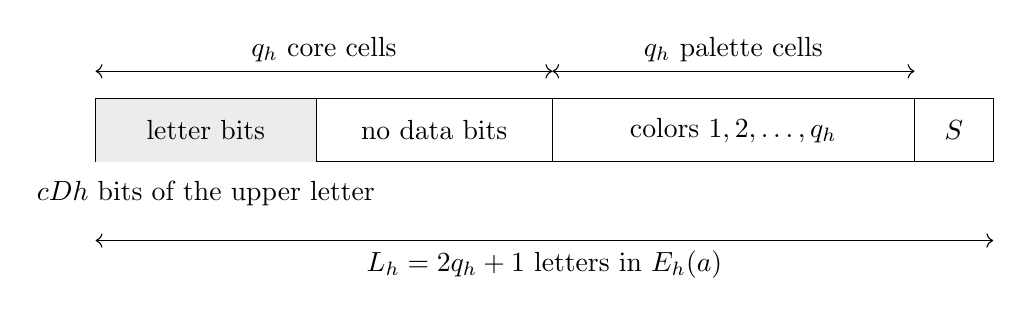
\begin{tikzpicture}[x=1cm,y=1cm]
 \draw (0,0) rectangle (11.4,0.8);
 \fill[gray!15] (0,0) rectangle (2.8,0.8);
 \draw (2.8,0)--(2.8,0.8);
 \draw (5.8,0)--(5.8,0.8);
 \draw (10.4,0)--(10.4,0.8);
 \node at (1.4,0.4) {letter bits};
 \node at (4.3,0.4) {no data bits};
 \node at (8.1,0.4) {colors $1,2,\ldots,q_h$};
 \node at (10.9,0.4) {$S$};
 \draw[<->] (0,1.15)--(5.8,1.15);
 \node[above] at (2.9,1.15) {$q_h$ core cells};
 \draw[<->] (5.8,1.15)--(10.4,1.15);
 \node[above] at (8.1,1.15) {$q_h$ palette cells};
 \node[below,align=center] at (1.4,-0.12) {$cDh$ bits of the upper letter};
 \draw[<->] (0,-1.0)--(11.4,-1.0);
 \node[below] at (5.7,-1.0) {$L_h=2q_h+1$ letters in $E_h(a)$};
\end{tikzpicture}
\caption{A canonical block encoding one letter $a\in\Sigma_{Dh}$.
The core carries its $cDh$ data bits, the palette contains each color
once in increasing order, and the stop cell closes the block. Both
control tracks are idle. The widths are schematic; the data positions
fit inside the core by the choice of $h_0$.}
\label{fr:block-figure}
\end{figure}


The replacements will carry out a proposed upper-level relation inside
one or more complete blocks. They temporarily acquire the cells of those
blocks, keeping the present data and a proposed replacement in separate
slots. The verifier checks a certificate for the proposed relation before
the replacement can become the represented data. We first specify the
control fields that keep this operation confined to its own cells.

\subsection{Control tracks and admissible neighboring pairs}

The palette-checker track has states
\[
 I,\qquad A_x,\qquad H_x\qquad(1\leq x\leq q_h),
\]
meaning idle, passed while seeking $x$, and the checker head seeking
$x$. The checker-head flag is set exactly in state $H_x$.
Within a palette the allowed adjacent checker-state pairs are
\[
 (I,I),\qquad (A_x,A_x),\qquad (A_x,H_x),
 \qquad (H_x,I).
\label{fr:checker-pairs}
\]
There is no restriction on the first palette state except its format;
the last palette state must be $I$ or $H_x$.  These are pair tests at
$C(q_h)P$ and $PS$.  They enforce a passed prefix, then its head, then
an idle suffix, or an entirely idle palette, whenever both ends of
the palette are present.  Truncated versions are allowed at the ends
of a word.

The transaction track is either idle or has one of the markers
\[
 L,\quad R,\quad B,\quad F.
\]
The first two are left and right wing markers; $B$ is a boundary
cursor and $F$ is a full verification head. The transaction-head flag
is set exactly on $B$ and $F$. Every nonidle transaction
letter carries metadata
\[
 (l,\tau,b),\qquad 1\leq l\leq k,\quad
 \tau\in\{\mathrm{rep},\mathrm{zero}\},\quad 1\leq b\leq l.
\]
Here $l$ is the intended number of blocks and $b$ is the relative
block number.  A head, and only a head, also carries a committed-side
bit $\epsilon$.  For a zero task $\epsilon=0$.  A full head carries
the verifier control and three reading bits described below.  A
boundary cursor has no verifier control or reading bits.  Wing
markers store neither a committed-side bit nor a verifier phase.

A core cell with a nonidle transaction track is called locked. It has
data slots numbered zero and one at positions $p\leq cDh$, and one
certificate bit at every core position. Palette and stop cells have
neither data slots nor certificate payload. These are unary format
requirements. In a replacement transaction, the two slots hold the
proposed source and target upper words. The side bit $\epsilon$ on the
head selects which slot currently represents the data of the acquired
cells. Acquisition copies the old data into that slot; release restores
the selected slot to the idle data field. Once acquisition has reached
the end of all $l$ blocks, full verification keeps both slots and the
certificate fixed. Only successful verification permits changing
$\epsilon$; reversing verification and releasing the cells then exposes
the other word. For a zero transaction only slot zero is tested, and
success will instead be declared zero.

These describe the intended use of the fields, not a restriction to
states reached by that use. The pair tests and moves below also specify
the meaning of arbitrary letters with those fields.

For a nonidle letter define its \emph{known first position} to mean
$b=1$ and structural type $C(1)$, and its \emph{known last position}
to mean $b=l$ and structural type $S$.  The following two unary zero
declarations are part of the table:
\begin{equation}\label{fr:endpoint-zero}
 R\text{ at its known first position is zero},\qquad
 L\text{ at its known last position is zero}.
\end{equation}
They depend on the letter itself and do not test for an absent word
neighbor.

Here is a complete specification of the transaction pair tests.  Give
each side of a letter a required interface, internal or external,
using the following table.  An internal interface also prescribes the
marker on the neighboring side.
\[
\begin{array}{c|c|c}
 \text{marker}&\text{left interface}&\text{right interface}\\ \hline
 \text{idle}&\text{external}&\text{external}\\
 L&\text{external at first; otherwise internal from }L
   &\text{internal to }L,B,F\\
 B&\text{external at first; otherwise internal from }L
   &\text{external}\\
 F&\text{external at first; otherwise internal from }L
   &\text{external at last; otherwise internal to }R\\
 R&\text{internal from }F,R
   &\text{external at last; otherwise internal to }R
\end{array}
\]
For each available neighboring pair its two facing interfaces must
both be external or must both be internal with the prescribed
markers.  In an internal pair, $l,\tau$ agree, $b$ is unchanged within
a block and increases by one across $SC(1)$, and the structural
adjacency is one in \eqref{fr:structural-pairs}.  No internal pair may
enter the known first position or leave the known last position.
External pairs still obey the structural adjacency test.  These rules
are precisely comparisons of the fields of the two letters.

In particular an external entrance into a locked region occurs only
at $C(1)$ with $b=1$.  A complete full region has the form $L^*FR^*$,
occupying its $l$ blocks; a boundary-cursor region has the form $L^*B$
and can stop at any acquired cell.  If it stops inside a block, the
rest of that block is idle.  Distinct regions can abut at a block
boundary.  Their metadata need not agree.  At the ends of the whole
word an interface for which no neighbor is present is not checked;
the unary exclusions \eqref{fr:endpoint-zero} continue to apply.

All violations of the structural, checker, or transaction pair tests
are elementary zero declarations of length two.  All unary format
violations are elementary zero declarations of length one.  This
specifies the syntax also for words that were never reached by a
computation.

\subsection{Palette operations}\label{fr:palette-operations}

The following replacements preserve every field not explicitly
changed.  Their instances are taken for every admissible value of
those fields.
\begin{enumerate}
\item At $C(q_h)P$, change an idle checker state on the palette cell
to $H_x$, with any $x$, and include the inverse replacement.
\item On two consecutive palette cells, replace the checker states
$H_x,I$ by $A_x,H_x$ if the color of the first cell differs from $x$;
include the inverse replacement.
\item Transpose the colors of two consecutive palette cells whose
other fields are identical, provided neither cell carries a checker
head or a transaction head.
\end{enumerate}
The following additional zeros are declared: a passed cell $A_x$ of
color $x$; two consecutive palette cells of the same color; and the
pair $P(a)S$ when the palette cell carries $H_x$ and $a\ne x$.
There are no other palette operations.  In the third operation the
non-color fields coincide, so transposing the colors is exactly
transposing the whole letters.

\begin{lemma}\label{fr:palette-soundness}
A complete palette containing each color exactly once, initially
idle on its checker track, cannot reach a palette zero under the
palette operations, interleaved arbitrarily with the transaction
operations defined below. Conversely, suppose a palette together with
its preceding $C(q_h)$ and following $S$ occurs in a nonzero word.
Its checker can be removed by replacements supported on those cells.
Once its transaction track is also idle, the palette has each color
exactly once and can be sorted into increasing color order.
\end{lemma}

\begin{proof}
The transaction operations leave all colors and checker fields in
place.  Palette operations preserve the multiset of colors.  During
a check for $x$, every passed cell has color different from $x$: this
is the condition for a forward step, and swaps within a passed run
preserve it.  A swap cannot cross from the passed region to the head
or idle region because their checker fields differ.  In particular,
if every color occurs, a head seeking $x$ cannot reach the last cell
with a different color after having passed all earlier cells.
Distinctness also prevents an equal-color adjacency.

For the converse, checker syntax in a complete palette either gives
an idle palette or gives a single head after a passed prefix.  If a
passed cell has the sought color the whole word is zero. Otherwise every
backward checker step is allowed.  Move the head back to the first
palette cell and apply the inverse creation rule using $C(q_h)$.
This does not require a transaction head to be in any specified
place.  With both tracks idle, all palette letters have identical
non-color fields.  Repeated colors can be brought adjacent by swaps,
and a missing color can be sought from the first cell to the last,
where the final test gives zero.  A nonzero palette therefore has
exactly one copy of each color, which can be sorted by adjacent
transpositions.
\end{proof}

\subsection{Acquisition and the local verifier}\label{fr:verifier}

For the moment fix any finite program code $a$.  At parameter $h$ the
verifier will test a certificate asserting that this program accepts
the proposed elementary rule at parameter $Dh$.  The certificate and
its addressable clauses will be specified in
Subsection~\ref{fr:tableau}.  All that is needed for the local moves
is a nonempty ordered list of clauses
\begin{equation}\label{fr:clause-list}
 \Phi_1,\ldots,\Phi_m,\qquad m\leq q_h,
\end{equation}
each reading at most three bits.  A bit address specifies either a
data slot, its relative block number and core position, or a
certificate bit in the first relative block.  Repeated addresses are
allowed.  Clauses with fewer than three inputs can be padded by
repeated inputs; a constant clause uses a dummy certificate address
whose value its truth function ignores.  The addresses and the truth function of an indexed
clause are computable from $a,h,l,\tau$ and the index.  They do not
depend on the committed side.  The tested input uses both data slots
for a replacement task and only slot zero for a zero task.

The acquisition replacements are the following.
\begin{enumerate}
\item An idle $C(1)$ can become a boundary cursor with $b=1$, with
chosen $l,\tau,\epsilon$.  Its previous data bit is placed in slot
$\epsilon$; its other data slot, when present, and its certificate
bit are chosen arbitrarily.
\item A boundary cursor can acquire its immediate next cell if that
cell is idle for transactions and would be an internal next position
of the chosen region.  The old cursor becomes $L$, the next cell
becomes the boundary cursor, and the metadata and side pass to the
new cursor.  On a core cell the old idle data are copied into the
committed slot and the other slot and certificate bit are chosen
arbitrarily.  Palette and stop cells acquire no payload.
\end{enumerate}
Both moves have their inverse moves and there are no other
acquisition or release moves.  Thus release returns the data in the
committed slot to the idle data field.  An acquisition cannot advance
beyond its known last position.  At that position, and only there,
its boundary cursor may become a full head in the initial verifier
state described next, with zero reading registers; this change also
has its inverse.

A full head holds $\epsilon$, a clause index when appropriate, a
phase tag from the following fixed list, and a register
$\rho\in\{0,1\}^3$.  For clause $j$ its control path is
\begin{equation}\label{fr:control-path}
 A_j\ \longleftrightarrow\
 \text{reading tour}\ \longleftrightarrow\ B_j^{\rm gate}
 \ \longleftrightarrow\ G_j^{\rm gate}
 \ \longleftrightarrow\ \text{undo tour}
 \ \longleftrightarrow\ Z_j.
\end{equation}
The symbols $B_j^{\rm gate}$ and $G_j^{\rm gate}$ here name verifier
phases, not boundary cursors.  The endpoint phases in
\eqref{fr:control-path} occur only at the known last position; this
is a unary format condition.  All eight register tuples are
syntactically allowed in every full-head phase.  A state $A_j$, $Z_j$,
or success with $\rho\ne0$ is declared zero.  These are semantic zero
declarations, not exclusions from the alphabet's syntactic formats.
Likewise a false after-gate state below is syntactically representable
but zero.  Replacement edges may have such zero-declared endpoints.
This distinction is essential: a forged tour must be able to reach a
zero-declared interface during rollback.  The initial acquisition
interface is $A_1$ with $\rho=0$.

Here are the complete movement conventions for both tours.  The
reading tour starts at the last position in a left-going phase.
A left move changes a neighboring transaction pair $L,F$ to $F,R$.
Each cell retains its payload, structural fields, and transaction
metadata $(l,\tau,b)$. Only the head's control phase, clause index,
committed-side bit $\epsilon$, and reading registers pass to the new
head position; the vacated cell loses these head-only fields.
Thus the relative block number at the new head is the number already
carried by that cell, including when the move crosses a block boundary.
For each address of clause $j$ located at the new head position, XOR
the bit at that address into its corresponding reading register.
If the cell is not an address, do nothing to the registers. At the
known first position a unary turn enters a right-going phase. Right
moves change $F,R$ to $L,F$ using the same field-transport convention
and do not read bits.  At the known last
position a unary exit enters $B_j^{\rm gate}$.  Each of these moves
has its exact inverse.  The tour's entry and exit edges preserve
every register tuple, including tuples making an endpoint a semantic
zero; they never reset a register.  The last position is a stop cell, which is
never a bit address, so the left-going convention reads every
addressed bit once and none is lost at the initial endpoint.

At $B_j^{\rm gate}$ the gate edge to $G_j^{\rm gate}$ exists exactly
when $\Phi_j(\rho)$ is true.  An after-gate state
$G_j^{\rm gate}$ with false $\Phi_j(\rho)$ is declared zero.  A
before-gate state with a false value has no gate edge but is not, for
that reason, zero.

The undo tour starts at $G_j^{\rm gate}$, travels left without
reading, turns at the first position, and travels right. On \emph{leaving}
a cell, it XORs each bit addressed there into its corresponding reading
register. It exits at the
last position into $Z_j$.  Its movement phases are distinct from the
reading-tour phases, and all its edges have their inverse edges.
Its entry and exit likewise preserve every register tuple, including
zero-declared endpoint states.
For $j<m$, a unary edge takes $Z_j$ to $A_{j+1}$ with zero registers.
For $j=m$ it takes $Z_m$ to a success phase, again with zero
registers.  The success phase is allowed only at the last position.
For a replacement task with zero registers a unary success edge changes $\epsilon$ to
$1-\epsilon$.  For a zero task the success phase is itself a unary
zero declaration.  There is no success-to-acquisition edge.  A
return to acquisition follows the inverses of
\eqref{fr:control-path} all the way to $A_1$.

Movement phases allow every position of the region, with clause
index in $\{1,\ldots,m\}$.  Every turn or entry or exit is a separate
unary phase change at its prescribed endpoint.  The only register
tests are the specified zero-register interfaces and the after-gate
tests.  This convention completely lists the control transitions;
there is no clock or phase stored on wing cells.

Each elementary move is a unary or two-letter replacement.  Take its
instances for every value of unaffected fields, preserving them
exactly, subject to the syntactic formats and the internal-pair
conditions on a pair used inside a region.  In an acquisition the
changed pair is tested as an internal pair after acquisition.  Every
zero mentioned so far is also unary or binary.  All strings of
lengths $3,\ldots,k$ have no elementary entries except in the
provisional small-parameter convention below.  The allowance of
$l\leq k$ in the verifier causes no problem when a task of arity
$l>2$ has no accepting input.  A semantic zero declaration never
removes an otherwise specified replacement edge.  The acquisition
interface, interclause edges, and edge from $Z_m$ to success retain
their explicitly specified zero-register condition.

\begin{lemma}\label{fr:context}
Starting from a concatenation of complete clean blocks, the
structural, transaction, and checker syntax is preserved under all
elementary replacements.  Distinct transactions never own cells of
the same block.  The elementary moves are context safe at both
untouched neighboring letters, even when two transaction regions
abut.
\end{lemma}

\begin{proof}
Structural tags never change, so structural syntax
is preserved.  For the transaction syntax it suffices to check the
interfaces of each kind of move.

If an idle $C(1)$ occurs in a syntactically admissible complete
configuration, its predecessor, if present, has an external right
interface.  The predecessor may be idle, a completed full region's
last letter, or a boundary cursor stopped at the preceding stop.
Its successor $C(2)$ is idle: a new locked region cannot start at an
internal core position.  Creating a boundary cursor therefore
preserves the external interface on each side.  This remains true
when the preceding boundary cursor intends to acquire more blocks.
It has not acquired this block, and its next acquisition is blocked
until the new cursor releases it.

In an acquisition, the old cursor becomes a left marker and its
idle successor becomes the new cursor.  Its untouched predecessor
previously permitted a left marker or a head with these same
metadata, and still does.  The new cursor has an external right
interface, as the old idle cell did.  If its untouched successor is
inside that block, the successor is idle, since a locked region
cannot start there; if it is a block start, it may also start a new
region, which is an allowed external joint.  The known-last
restriction prevents acquisition from creating the prohibited last
left marker.  The inverse release has the same interface checks in
reverse.  At $C(1)$ inverse creation is possible only for a boundary
cursor with no acquired successor, so it too preserves the outside
interfaces.

In a full movement $F,R\leftrightarrow L,F$, the exterior
predecessor permits respectively $F$ or $L$, and the exterior
successor permits respectively $R$ or $F$.  Their internal metadata
are unchanged.  A move cannot introduce a right marker at first or
a left marker at last because the old head must have the indicated
neighbor inside its region.  Endpoint phase changes do not change
these interfaces.  The boundary-to-full change is at the last
position, where both heads have an external right interface and the
same left-interface requirement.  Changing the committed side at
success changes no interface at all.

For the checker track, head creation occurs at its first position
with an idle next checker cell, if present.  A forward step changes
$H_x,I$ to $A_x,H_x$ and has the prescribed predecessor and successor
in the checker grammar.  Its inverse has the same property.
Palette swaps preserve both marker tracks, since their non-color
fields must coincide.  The main moves leave checker fields and
colors in place; checker moves leave main fields and payload in
place.  In particular a main head may cross a checker head without
any additional interface change.

Finally any acquired part of a block includes its $C(1)$, or is a
continuation of a region that acquired that $C(1)$ earlier.  Creation
is allowed only at an idle $C(1)$, and acquisition takes only idle
cells.  Since the only idle suffix of a partially acquired block is
strictly after its cursor, no other transaction can start in that
suffix or enter it from the left.  This proves the ownership claim
and completes the induction over replacements.
\end{proof}

For configurations reached from clean blocks, the context lemma ensures
that a full transaction keeps its data and certificate fixed even when
operations elsewhere are interleaved with its verification. For a fixed
payload, the control path has two
properties. A head started at its acquisition interface checks the
clauses correctly; an arbitrary full-head state can be undone or exposes
a zero. The second property is needed for words that did not start clean.

\begin{lemma}\label{fr:verification}
Fix the data slots and certificate of a complete syntactically admissible
transaction region.
Using only full-head control moves and starting at $A_1$ with zero
registers, a full head can reach success
precisely when every clause is true on those fixed bits. No such path
reaches a format, nonblank-register, or false-after-gate zero. After a
replacement success changes the committed side, verification can be
reversed to the acquisition interface.
\end{lemma}

\begin{proof}
The tour edges are invertible. Starting at $A_j$ with zero registers,
the reading tour reaches its gate with exactly the three bits from
the clause's addresses, and the undo tour restores zero registers.
A false gate breaks the path before its after-gate state.
Backtracking cannot circumvent this break: the only changes of clause
index are the specified edges from $Z_j$ to $A_{j+1}$, the only
acquisition interface is $A_1$, and the only extra success edge changes
a side bit which the schedule does not read. Thus success is reached
exactly when all clauses are true, and no format, nonblank-register,
or false-after-gate zero is reached. After a side change, the same
clauses still read the same fixed slots, independently of the selected
side, so all verification moves can be reversed.
\end{proof}

\begin{lemma}\label{fr:rollback}
A complete transaction region with one full head in any allowed
control state can either be returned to acquisition by replacements
inside the region, or can reach a declared zero there.  This remains
true when its control state and registers were not reached from
acquisition.  A boundary-cursor region can always be released inside
its acquired interval.
\end{lemma}

\begin{proof}
Fix the payload of the region.  Each tour edge is a bijection on
register tuples: it is either the identity or XOR by a specified
tuple of the fixed payload bits.  The legs and turns give a
prescribed finite path.  From any interior tour position, reversing
that path reaches the endpoint preceding the tour, regardless of
the initial register tuple.  The endpoints exist because this is a
complete region.

For a reading tour this returns to its $A_j$ endpoint, where a
nonzero register tuple is zero by declaration.  For an undo tour it
returns to $G_j^{\rm gate}$.  If the gate predicate there is false,
the word is zero.  Otherwise cross the gate backward and reverse
the reading tour, again reaching $A_j$ or zero.  The same argument
starts directly from either gate phase.  In particular a false
before-gate value is not a trap: it can reverse its reading tour.

From $A_j$ with $j>1$, reverse the edge from $Z_{j-1}$ and apply the
same argument to the preceding clause.  A success state first
reverses to $Z_m$; its registers must already be zero, or it is a
declared zero.  Thus the clause index decreases until $A_1$ is
reached, or a specified violation occurs.  No argument assumes that
an earlier clause has actually been checked.  The reverse gate
test and the required blank-register endpoints supply precisely
the checks needed for arbitrary starting states.

At $A_1$ reverse the boundary-to-full change.  Inverse acquisition
then moves the boundary cursor back through its acquired prefix,
returning committed data to the idle cells; finally inverse
creation removes it.  None of these moves reads a cell outside the
acquired interval.  The same release argument applies immediately
to a region already carrying a boundary cursor.
\end{proof}

\subsection{An addressable computation tableau and the fixed point}
\label{fr:tableau}

The moves above use a finite list of three-bit tests. We now produce
that list from a computation deciding membership in the next-level
rule table. Encoding an accepting computation by local Boolean
constraints is the computation-tableau method used in Cook's theorem
\cite[proof of Theorem~1]{Cook1971}. Here we specify the addresses and size bounds
needed by the word rules.

We specify the clauses in \eqref{fr:clause-list}.  Fix once and for
all a deterministic universal one-tape machine with a fixed finite
tape alphabet and state set.  It is arranged to simulate a supplied
program code, to return its head to a distinguished origin when
accepting, and then to remain frozen.  The simulation and the return
to the origin have polynomial overhead for every fixed simulated
program.  One explicit implementation stores the simulated tapes
and head marks on tracks and scans their used portions to implement
each simulated step; the used portions grow at most linearly in
the number of simulated steps.  A fixed binary interpreter handles
the finite program code.  Such scans give polynomial, rather than
an assumed constant, simulation overhead, which is all that is
needed here.

Put
\[
 T=2^{\lfloor h/5\rfloor},\qquad W=4T,\qquad o=2T.
\]
Use time rows $0,\ldots,T-1$ and tape positions $0,\ldots,W-1$,
with the marked origin at $o$.  Encode each tape symbol, origin
marker, and possible head state with $\beta$ bits, where $\beta$ is
an absolute constant.  Let
\[
 \operatorname{enc}(n)=1^{|\operatorname{bin}(n)|}
                 0\operatorname{bin}(n)
\]
for a nonnegative integer $n$, with $\operatorname{bin}(0)=0$.
The initial tape, starting immediately to the right of the
origin, contains
\[
 \operatorname{enc}(|a|)\,a\,
 \operatorname{enc}(Dh)\,\operatorname{enc}(l)\,
 \operatorname{task}(\tau)\,\operatorname{data}.
\]
The data are the $lcDh$ bits in slot zero, ordered by block and
core position, followed, for a replacement task, by the same list
from slot one.  All other initial cells are fixed, including the
initial head and blank cells.  Each bit coordinate of a cell
encoding one input bit is a constant, that input bit, or its
negation.  Take $h$ large enough that this input occupies fewer
than $T/4$ tape positions.  Neither the input nor a head starting
at the origin can reach the boundary cells in fewer than $T$
steps.

A deterministic tape-machine step has a radius-one description:
the new symbol and head label at a cell are determined by the
previous labels at that cell and its two neighbors.  Extend this
map arbitrarily on inconsistent three-cell patterns to a total
Boolean function
\[
 f:\{0,1\}^{3\beta}\longrightarrow\{0,1\}^{\beta}.
\]
Fix a NAND circuit for $f$ with $g$ gates.  Both $\beta$ and $g$
are independent of $a,D,h$.  The initial row is a valid one-head
configuration, so the arbitrary values on inconsistent patterns
will not be used in a satisfying tableau.

Allocate certificate variables $X(t,j,r)$ for all tableau bits,
and $Y(t,j,v)$ for the auxiliary circuit gates, with exact
one-based core addresses
\begin{align*}
 X(t,j,r)&:\quad 1+\beta(Wt+j)+r,
 &&0\leq t<T,\quad 0\leq j<W,\quad 0\leq r<\beta,\\
 Y(t,j,v)&:\quad
 1+\beta WT+g((W-2)t+j-1)+v,
 &&0\leq t<T-1,\quad 1\leq j<W-1,\quad 0\leq v<g.
\end{align*}
The total number of certificate variables is
\begin{equation}\label{fr:certificate-count}
 \beta WT+g(W-2)(T-1).
\end{equation}
List the following clause families in the displayed order, using
lexicographic order of their coordinates within each family.
\begin{enumerate}
\item For each initial-row bit use two clauses.  A prescribed
constant uses its unit clause twice; equality to an addressed
data bit $x$, or to its negation, uses the two clauses expressing
that equality.
\item For every later time and each of the two boundary cells,
use one unit clause per bit, keeping that cell blank.
\item For each pair $(t,j)$ with $t<T-1$ and $1\leq j<W-1$,
encode the $g$ NAND gates in order.  The equation
$z=\neg(u\wedge v)$ uses the three clauses
\[
 (u\vee z),\qquad(v\vee z),\qquad
 (\neg u\vee\neg v\vee\neg z).
\]
Here the circuit inputs are the appropriate neighboring
variables $X(t,j-1,r),X(t,j,r),X(t,j+1,r)$ and the preceding
gate variables at $(t,j)$.  Add two clauses for each of the
$\beta$ circuit outputs to equate it to the corresponding
$X(t+1,j,r)$.  Thus this family has exactly $3g+2\beta$ clauses
per $(t,j)$.
\item Use $\beta$ unit clauses fixing the final cell at the
origin to the accepting head state and its fixed origin symbol.
The universal machine is arranged to leave that symbol fixed
when it accepts and freezes.
\end{enumerate}
Constants on circuit wires are allowed; clauses containing them
are interpreted as Boolean functions of the remaining inputs.
Use repeated literals, or an ignored dummy input for a constant
function, to supply the three reading addresses.  The number of
clauses is exactly
\begin{equation}\label{fr:clause-count}
 2\beta W+2\beta(T-1)
 +(3g+2\beta)(W-2)(T-1)+\beta.
\end{equation}

The clauses force a unique next row from the preceding row, with
the correct gate values.  Induction from the valid initial row
therefore makes every satisfying tableau the actual computation
of the universal machine.  The fixed blank boundaries do not
alter it, since the head cannot reach them.  The final constraint
is satisfied exactly when the computation accepts before time
$T$; an earlier acceptance extends to the final row by freezing.
Conversely every such accepting computation, with its circuit
gate values, gives a satisfying certificate.

The four family sizes and the formulas for their addresses are
explicit.  Comparison with the four cumulative sizes followed
by quotient and remainder recovers from one clause index its
family, time, position, and bounded subindex.  The gate circuit
is fixed.  Initial-row lookup selects a bit of the fixed code, a
parameter bit, a delimiter, or one addressed data bit.  Thus one
clause and its at most three addresses are generated in time
polynomial in $h$ for fixed $a,D$, using $O(h)$-bit arithmetic.
No preceding clauses or complete tableau are enumerated.

Both \eqref{fr:certificate-count} and
\eqref{fr:clause-count} are $O(T^2)$ with absolute constants,
so for all sufficiently large $h$ they are at most $q_h$.
Store the entire certificate in the first relative core, in its
first required number of certificate positions.  Any unused
certificate bits have no effect.  Thus the only nonconstant
quantities on a verifier head are its $O(h)$-bit clause index and
the already listed metadata and three reading bits.  Code $a$, the
next-level letters, and the tableau are not head fields.

We now remove the apparent reference to an unspecified program.
For a provisional code $a$, let
\[
 P(a,h;l,\tau,\text{candidate data})\in\{0,1\}
\]
be the following finite predicate.  Decode the candidate one- or
two-sided string of $l$ letters of length $ch$ and decide whether
it is an elementary table entry described in
Subsections~\ref{fr:formats}--\ref{fr:verifier}, using the tableau
with initial program code $a$ just specified.  For replacements
accept either orientation of every listed move.  For zeros use
the listed unary and binary declarations.  For all other proposed
entries return zero.  Format zeros include illegal letter formats;
replacement entries always have the specified syntactic fields on
both sides.  The additional semantic register and gate zeros do not
exclude these fields or suppress any specified replacement entry.
If the parameter is too small for any of the declared
encodings, input layout, clause count, or certificate count to fit,
use instead the trivial table declaring every one-letter word
zero and having no replacements.  These fit conditions are
integer inequalities in the explicit layout sizes.

This predicate is computable in time polynomial in $h$ for fixed
$a,D$.  A syntax test compares a bounded number of fields.  A
movement test checks the indicated changed bits and, if needed,
generates the addresses for its one clause.  An after-gate test
evaluates one three-input truth function on the head registers.
The predicate never asks whether a tableau exists and never
executes the program $a$.  It merely uses the finite string $a$ as
part of the prescribed time-zero data.

We use Kleene's fixed-point construction in the self-simulation
setting developed by Durand, Romashchenko, and Shen, where
polynomial-time local checks are also explicit
\cite[Section~2.3]{DurandRomashchenkoShen2012}. The simulation overhead
and clause-address computation for the present implementation must
still be checked, as above and below.

For completeness, the fixed-point construction can be given at
the level of finite programs.  There is an effective constructor
$s(t,v)$ for a code that, on input $x$, simulates the two-input
program $t$ on $(v,x)$.  A fixed wrapper obtains polynomial
simulation overhead by the scanning implementation just described.
Let $t$ be the two-input program which, on first input $v$, forms
the finite code $s(v,v)$ and, on remaining input $x$, computes
$P(s(v,v),x)$.  Set
\begin{equation}\label{fr:fixed-point}
 a=s(t,t).
\end{equation}
Then the program $a$ returns $P(a,x)$ for every input.  With this
particular $a$ fixed, forming $s(t,t)$ is a constant cost; evaluation
of $P$ and the fixed wrapper have polynomial running time in $h$.
There is no recursive call to $a$ during evaluation of $P$.

Choose $D$ before making \eqref{fr:fixed-point}.  The program $a$
then has a polynomial running-time bound at parameter $Dh$, with
constants allowed to depend on the fixed $D,a$.  Since $T$ grows
exponentially in $h$, choose $h_0$ so large that for every $h\geq h_0$
all field and layout bounds hold, and every such computation,
including universal simulation and return to the origin, finishes
strictly before $T$.  In particular an input has an accepting
tableau exactly when it is an elementary table entry at parameter
$Dh$.  This is the desired finite, nonrecursive definition of all
the tables.  No increase of $c$ or $k$ depends on $D$ or on the
length of $a$.

\subsection{Faithful simulation on clean words}\label{fr:simulation}

We now combine the local verifier with the fixed point. An accepting
certificate exists exactly for an elementary rule at parameter $Dh$.
We show that the canonical encoding $E_h$ simulates each such rule and
that arbitrary lower-level replacements cannot destroy a nonzero
encoded word.

\begin{lemma}\label{fr:faithful}
The substitution $E_h$ simulates every elementary next-parameter
replacement and zero declaration.  Moreover, if $w$ is a nonzero
word at parameter $Dh$, no sequence of lower-parameter
replacements starting from $E_h(w)$ can reach a zero declaration.
\end{lemma}

\begin{proof}
For an elementary replacement on $l$ letters, acquire the $l$
canonical blocks with the source data in the committed slot, the
target data in the other slot, and an accepting computation
certificate in the first core.  All required acquisitions exist.
The verifier checks every clause, reaches success, changes the
committed side, and follows inverse verification and release moves
to leave the target blocks.  Their palettes and checker tracks
have not changed.  The same procedure for an elementary zero
declaration uses its accepting certificate and reaches the
success zero.  No cell outside those blocks is needed.

For the converse, consider any sequence from a concatenation of
canonical blocks.  By Lemmas~\ref{fr:context} and
\ref{fr:palette-soundness}, all structural and marker syntax
remains valid and all palettes retain exactly one of each color.
At any time read a represented higher-level word as follows.  An
idle core cell contributes its idle data bit.  An acquired core
cell contributes the data bit in the side selected on its region's
unique head.  The ownership assertion in Lemma~\ref{fr:context}
makes this unambiguous.  Acquisition and release preserve the
represented word, even when they choose new uncommitted data or
certificate bits after a partial release.  Palette operations do
not affect it.

While a head is full, every slot and certificate bit of its
region is fixed. Interleavings with another transaction cannot change
this payload, by ownership; palette operations cannot change an
addressed bit. Lemma~\ref{fr:verification} therefore applies throughout
the transaction. If it reaches replacement success, its certificate
establishes a genuine elementary rule on the currently represented
letters. Changing the selected side changes the represented word by
precisely that rule, and subsequent backtracking remains valid.
A reached zero-task success likewise establishes an elementary zero
on the currently represented word. No format, nonblank-register, or
false-after-gate zero can be reached by verification started from
acquisition.

These statements induct over the arbitrary sequence of
replacements.  All represented words are replacement-equivalent
to the starting word.  If that word is nonzero, a simulated zero
success is impossible; all other zero declarations have already
been excluded by the invariants.  This proves nonzero
preservation.  Complete initial blocks keep all transaction
regions complete; an absent neighbor can only prevent a requested
acquisition, never supply a new transition.
\end{proof}

A legal idle letter $C(p)$ at a middle core position $1<p<q_h$
is a nonzero one-letter word.  It is neither a unary zero nor the
site of unary cursor creation, and no two-letter move applies to
it.  Such a position exists after increasing $h_0$.  In particular,
iterating Lemma~\ref{fr:faithful} a finite number of times produces
nonzero words of unbounded lengths at any fixed level.  This
observation does not require taking an infinite word or an infinite
presentation.

\subsection{Arbitrary words, cuts, and isolated normalization}
\label{fr:tokens}

It remains essential to control words that do not begin clean. Here
we use rollback in the opposite direction: any complete transaction
appearing in a nonzero word must admit release, since exposing a zero
inside that transaction would make the whole word zero.
Declare a cut immediately before $C(1)$ if its transaction track
is idle or has relative block number 1.  This is a condition on
one letter.  In a locally admissible word it marks either an idle
block beginning or the beginning of a transaction's first block.
In particular the unary exclusion of a right marker at a known
first position prevents a headless right wing from masquerading
as such a beginning at the left end of the whole word.

\begin{lemma}\label{fr:fragment-bound}
There is a bound depending only on $h$ for every palette fragment
in a nonzero word.  One may take $16q_h+2$.  An interval without a
cut has bounded length depending only on $h$, including when the
interval reaches an end of the word.
\end{lemma}

\begin{proof}
There is no transaction start strictly inside a palette.  Its
transaction track has at most one head and otherwise consists
of constant-metadata wings, with a possible idle suffix after a
boundary cursor.  The checker track likewise has at most one
head and constant passed and idle runs.  The common refinement
of these two ordered partitions, after removing their at most
two head positions, has at most 16 homogeneous non-head
intervals.  This deliberately loose absolute bound also covers
fragments with one or both ends missing.  No payload is present
on palette cells, and their relative block number is constant
within an acquired part, so these intervals have identical
fields except for color.

If a color repeats inside such an interval, adjacent
transpositions bring its two occurrences together, producing an
equal-color zero.  Hence each interval in a nonzero word has at
most $q_h$ cells.  The asserted palette bound follows.  A whole
block, or either of its fragments, therefore has length at most
$17q_h+3$.

At successive core beginnings an acquired region's relative
number strictly increases until at most $k$, unless a new
transaction or idle block begins; the latter creates a cut.
There is no other possible continuation, by the internal and
external interface tests.  Thus an interval with no cut contains
at most $k$ intervening blocks, apart from its two end
fragments.  For example
\[
 B_h=(k+2)(17q_h+3)
\]
bounds every such interval.  This argument uses available pair
tests and the unary known-endpoint exclusions, not tests for
missing word neighbors.
\end{proof}

\begin{lemma}\label{fr:token-normalization}
An interval between consecutive cuts in a nonzero word consists
of between one and $k$ complete structural blocks and can be
changed, using only replacements inside that interval, to a
concatenation of canonical blocks.
\end{lemma}

\begin{proof}
The interval begins at $C(1)$ and ends at $S$, because the next
cut is another $C(1)$.  If its first block is idle, there can be
no locked start inside that block, and the next block would
give a cut.  The interval is then just one idle block.  Otherwise
its first nonidle letter has relative block number 1 and is
$L$, a boundary cursor, or a full head; it cannot be $R$ by
\eqref{fr:endpoint-zero}.

Starting with a left marker, follow its internal successors.
The chain cannot stop at an external interface, cross the next
cut, or end at the known last position, where a left marker is
forbidden.  It must therefore reach a head inside the interval.
A boundary cursor ends the acquired prefix; its remaining
current block is idle, and any later block would begin a new
interval.  A full head forces a right wing as far as its known
last position.  The interfaces admit no second head on that
wing.  This proves that a nonidle interval contains exactly one
transaction and at most $k$ blocks, including the final block
if acquisition stopped partway through it.

Every palette here is complete.  First remove all its checker
heads using Lemma~\ref{fr:palette-soundness}, or obtain a zero.
Apply Lemma~\ref{fr:rollback} to the transaction head and release
the acquired cells, or again obtain a zero.  The interval is a
factor of a nonzero word, so any sequence producing zero in the
interval would produce zero in that word and is impossible.
All these operations are thus successful replacements. Their support
is inside the interval: checker removal stays in the palette and its
preceding core cell, and release uses only the acquired prefix. Unlike the
clean-start argument, this step does not require the initial control
state to have been reached by acquisition.

The interval is now idle on both tracks.  In each palette a
missing or repeated color would give zero by
Lemma~\ref{fr:palette-soundness}.  Each palette has exactly
$q_h$ cells and can be sorted.  The remaining idle core data
specify one bit string of length $cDh$ per block.  These are
letters of the upstairs bit-string alphabet, including its
unused formats when considered before imposing its unary zero
relations.  The resulting word is exactly $E_h(u)$ for the
corresponding string $u$ of between one and $k$ letters.
\end{proof}

To finish the proof of Proposition~\ref{prop:hierarchy}, the alphabet
$\Sigma_h$ has the required cardinality $2^{ch}$, and the tables
just constructed are finite and have length
at most two, in particular at most $k=10$.
Property~\ref{fr:prop-encoding} follows from
Lemma~\ref{fr:faithful} and the nonzero middle-core letter.

For Property~\ref{fr:prop-tokens}, take as tokens the nonzero
intervals with the syntax in Lemma~\ref{fr:token-normalization}.
There are only finitely many: each has at most $k$ blocks and
each block has the bound in Lemma~\ref{fr:fragment-bound}.
For each token fix one of the normalizations furnished by
Lemma~\ref{fr:token-normalization} and denote its upstairs word
by $u_t$.  A cleaned block has $q_h$ core cells, $q_h$ palette
cells and one stop cell, so length preservation gives
$|t|=(2q_h+1)|u_t|$.  Every sufficiently long nonzero word has
at least two cuts by Lemma~\ref{fr:fragment-bound}; its prefix
before the first and suffix from the last have length at most
$B_h$.  All intervening intervals are tokens, and the
letter-recognized cuts make the decomposition unique.  The
normalizations take place in isolated intervals; no exterior
head, palette cell, or boundary test has been used.

Finally, every complete palette in a nonzero token has length
$q_h$ even before normalization, since its normalization
preserves length and structural tags.  Its at most two head
singletons and at most 16 homogeneous non-head intervals
therefore include an eligible run of length at least
$(q_h-2)/16$, hence at least $q_h/100$ for the chosen parameters.
A sufficiently long nonzero word has a token and such a
palette.  Swappability is an explicit table entry, and every
eligible run has distinct colors by the duplication argument
in Lemma~\ref{fr:fragment-bound}.  Its non-color tuple also
determines its maximal endpoints.  This proves
Property~\ref{fr:prop-runs} and completes the Proposition.

\section{Cancellation and the matrix-nil algebra}
\label{sec:cancellation}

We now use the hierarchy of Proposition~\ref{prop:hierarchy} to
construct the algebra needed for the group argument.  Fix its absolute
constants $c,k$, choose an integer
\begin{equation}
  D>10(c+1)(k+1),
  \label{ca:D}
\end{equation}
and then perform the program construction in that proposition and choose
$h_0$ sufficiently large.  Thus $D$ is fixed before the program fixed point
and before $h_0$.  Throughout this section put
\[
  h_j=h_0D^j,\qquad q_j=2^{h_j},\qquad
  L_j=2q_j+1,\qquad \Sigma_j=\Sigma_{h_j}.
\]
In particular $|\Sigma_j|\leq 2^{ch_j}$.  Write $A_j(K)=A_{h_j}(K)$ for
the algebra at level $j$ over a field $K$ of characteristic two, and write
\[
  E_j:A_{j+1}(K)\longrightarrow A_j(K)
\]
for the homomorphism induced by the block substitution $E_{h_j}$.  The
same symbol denotes that substitution on words.  Each upper letter is
replaced by a word of length $L_j$.

For a word $w$ on $\Sigma_j$, let $[w]_j$ denote its algebra image.  The
empty word has image $1$.  Scalar extension gives
$A_j(K)=K\otimes_{\F_2}A_j(\F_2)$: the defining relations have coefficients
in $\F_2$, and tensoring vector spaces over $\F_2$ is exact.  In particular
a nonzero word over $\F_2$ remains nonzero over $K$.  We use the usual
identification
\[
  M_d(K)\otimes_K A_j(K)=M_d(A_j(K)).
\]
Thus a numerical matrix commutes with an algebra element when the latter
is placed in every diagonal position, but numerical matrix factors retain
their original order.

\subsection{Weighted sums and matrix powers}

A matrix with entries in the positive-degree part of $A_j(K)$ has a
finite expansion
\[
 T=\sum_{\gamma\in\mathcal C}
 A_\gamma\otimes[v_\gamma]_j,
 \qquad A_\gamma\in M_d(K),\quad |v_\gamma|\geq1.
\]
Each term in $T^a$ is indexed by a sequence of $a$ summands, whereas its
total word length is the sum of the lengths of their labels. This length
can vary among terms in the same power. We first prove
cancellation after grouping such sequences by total word length. The
final subsection will recover cancellation at each sufficiently large
fixed number of factors.

\begin{definition}[Weighted tests]
\label{ca:tests}
A \emph{letter test} of dimension $d\geq1$ at level $j$ assigns a matrix
$M(a)\in M_d(K)$ to each $a\in\Sigma_j$.  For
$w=a_1\cdots a_n$ put $M(w)=M(a_1)\cdots M(a_n)$ and $M(\varnothing)=1_d$.
Its length-$n$ sum is
\begin{equation}
  S_{j,n}(M)=\sum_{w\in\Sigma_j^n} M(w)\otimes[w]_j.
  \label{ca:letter-sum}
\end{equation}
A \emph{chunk test} of dimension $d$ and label bound $b\geq1$ consists of
a finite set $\mathcal C$ of chunk identifiers, a nonempty label
$v_\gamma\in\Sigma_j^*$ with $|v_\gamma|\leq b$ for each
$\gamma\in\mathcal C$, and a weight $W_\gamma\in M_d(K)$.  Its length-$n$
sum is
\begin{equation}
  C_{j,n}(\mathcal C,W)=
  \sum_{\substack{r\geq0,\ \gamma_1,\ldots,\gamma_r\in\mathcal C\\
                   |v_{\gamma_1}|+\cdots+|v_{\gamma_r}|=n}}
  W_{\gamma_1}\cdots W_{\gamma_r}
       \otimes[v_{\gamma_1}\cdots v_{\gamma_r}]_j.
  \label{ca:chunk-sum}
\end{equation}
The empty sequence contributes $1_d\otimes1$ when $n=0$.
A test \emph{eventually vanishes} if its length-$n$ sum is zero for every
sufficiently large integer $n$.
\end{definition}

Different chunk identifiers may have the same label.  Moreover, different
sequences may spell the same word with different segmentations.  All such
sequences occur separately in Equation~\eqref{ca:chunk-sum}.  The sums are
finite because every label has positive length. For a letter test,
the length-$n$ sum is exactly a matrix power:
\[
 S_{j,n}(M)=\left(\sum_{a\in\Sigma_j}M(a)\otimes[a]_j\right)^n.
\]
For longer chunk labels, the length-$n$ sum instead includes sequences
with different numbers of factors. Unless a different bound is specified,
a chunk test below has label bound $k$.

\subsection{Cancellation inside one palette run}

The cancellation estimate uses an elementary alternating-multilinear
argument. Its dimension bound is sufficient for the hierarchy below.

\begin{lemma}[Alternating matrix sum]
\label{ca:alternating}
For a field $K$ of characteristic two and matrices
$X_1,\ldots,X_m\in M_d(K)$, put
\[
  \mathcal A_m(X_1,\ldots,X_m)
   =\sum_{\sigma\in S_m}X_{\sigma(1)}\cdots X_{\sigma(m)}.
\]
If $m>d^2$, then $\mathcal A_m(X_1,\ldots,X_m)=0$.
\end{lemma}

\begin{proof}
The map $\mathcal A_m$ is multilinear.  If $X_i=X_j$ with $i\ne j$,
pair a permutation $\sigma$ with $(i\ j)\circ\sigma$.  The two products
are equal, and the pairing has no fixed point.  Their sum is zero in
characteristic two.  Hence $\mathcal A_m$ is alternating, meaning that
it vanishes whenever two arguments agree.  Expand its arguments in a
basis of the $d^2$-dimensional vector space $M_d(K)$.  If $m>d^2$, each
term in the multilinear expansion has a repeated basis argument and is
therefore zero.  This proves the result without any division by $m!$.
\end{proof}

\begin{lemma}[Direct cancellation]
\label{ca:direct}
Fix $j,d,b$.  If
\begin{equation}
  \frac{q_j}{100}>b(d^2+3),
  \label{ca:direct-bound}
\end{equation}
then every dimension-$d$ chunk test of label bound $b$ at level $j$
eventually vanishes over every field of characteristic two.
\end{lemma}

\begin{proof}
Fix such a test and choose $n$ above the long-word threshold in
Proposition~\ref{prop:hierarchy}.  In its length-$n$ sum discard the
sequences whose concatenated word is zero.  We partition the remaining
sequences into permutation orbits and prove that each orbit contributes
zero.

For each remaining sequence let $w$ be its concatenated word.  Erase only
the color field from each letter of $w$, retaining its position and all
other fields. Among the maximal eligible runs, choose the first one
having length at least $q_j/100$. This choice exists by
Proposition~\ref{prop:hierarchy} and depends only on the color-erased
word.  Every eligible run in a nonzero word has distinct colors: if two
colors agreed, adjacent transpositions within that run could bring them
together and give a declared zero substring.  This also explains why
color distinctness need not enter the rule selecting the run.

Mark the chunk boundaries of the sequence.  Its \emph{packet} is the
consecutive list of all complete chunks contained in the chosen run.
Keep all other chunks fixed, including any chunk crossing an endpoint of
the run.  There are at most two crossing chunks.  If the run has length
$r$ and the packet contains $m$ chunks, then
\[
  r\leq mb+2b,\qquad
  m\geq r/b-2>d^2.
\]
Here the last inequality follows from Equation~\eqref{ca:direct-bound}.
In particular the packet is nonempty.

Permute these $m$ whole chunks arbitrarily.  They may have unequal
lengths, but their total length is fixed.  Thus the packet occupies the
same letter interval after every permutation, and every letter in that
interval retains the common non-color tuple.  The color-erased word is
unchanged at every position.  Consequently the chosen maximal run is
unchanged.  The exterior chunks, including the endpoint-crossing chunks,
are unchanged as well, so the complete chunks in this run are again
exactly the packet just permuted.  Its internal chunk boundaries may
move; its endpoints and the rule selecting it do not.

All words obtained in this way have the same algebra image: arbitrary
permutations of their letters within the run are products of the allowed
adjacent transpositions.  If any permuted word were zero, their common
image would be zero and the starting word would also be zero.  Thus the
discarded zero sequences cannot remove any member of a nonzero orbit,
and every permuted sequence is still among the summands under
consideration.  Conversely applying
the same procedure to any of them produces the same set of sequences.
These sets are therefore a partition into orbits.

The labels of the packet chunks are pairwise distinct.  Indeed each
begins with a different color, since their first letters occupy distinct
positions of the distinct-color run.  Hence the chunk identifiers in the
packet are also pairwise distinct, even if the original list admitted
several identifiers with a common label.  All $m!$ permutations give
different sequences of identifiers; the orbit is a free permutation
orbit.  This assertion concerns sequences, not their concatenated words.
Distinct segmentations of a word remain separate summands and belong to
their respective orbits.

Choose one orbit and write its fixed exterior matrix products as $U,V$,
the packet weights as $X_1,\ldots,X_m$, and its common algebra image as
$a\in A_j(K)$.  Its entire contribution is
\[
  U\left(\sum_{\sigma\in S_m}
      X_{\sigma(1)}\cdots X_{\sigma(m)}\right)V\otimes a.
\]
The weights $X_i$ themselves need not be distinct.  The displayed middle
sum vanishes by Lemma~\ref{ca:alternating}.  There are only finitely many
sequences of total length $n$, so summing the zero orbit contributions
proves the desired vanishing.
\end{proof}

\subsection{Moving a test to a larger palette}

Direct cancellation applies when the palette is large compared with the
test dimension. The fixed palette at level zero cannot meet
Equation~\eqref{ca:direct-bound} for every dimension. We first treat a
letter test by moving it to the next level, where the palette is larger.
The cuts turn
it into a chunk test on the bounded upper words attached to tokens. The
matrix automaton then turns such a chunk test back into a letter test, so
that the passage to the next level can be repeated. We keep track of the
increase in dimension and apply direct cancellation as soon as its
inequality holds for an incoming chunk test. The automaton will also
reduce any level-zero chunk test to a letter test, thereby covering the
longer labels in the original matrix expansion.

\begin{lemma}[Reduction by the cuts]
\label{ca:cut-reduction}
Fix a level $j$, a field $K$ of characteristic two, and a dimension $d$.
If every dimension-$d$ chunk test of label bound $k$ at level $j+1$
eventually vanishes, then every dimension-$d$ letter test at level $j$
eventually vanishes.
\end{lemma}

\begin{proof}
Let $M$ be a letter test at level $j$.  By
Proposition~\ref{prop:hierarchy}, there are integers $B,N_0$ such that
every nonzero word of length at least $N_0$ has the stated cut
decomposition, with initial and final pieces of length at most $B$.
Increase $B$ to at least one.  A cut is recognized solely from the letter
immediately after it; there is no additional cut after the last letter of
the word.

Take the token list $\mathcal T$ to be a set of distinct literal words.
For each $t\in\mathcal T$ fix once and for all an upper word $u_t$ with
\begin{equation}
  1\leq |u_t|\leq k,\qquad
  |t|=L_j|u_t|,\qquad [t]_j=E_j([u_t]_{j+1}).
  \label{ca:token-normalization}
\end{equation}
If a token has more than one possible upper normal form, choose one;
it is the literal token, not its normal form, that indexes this list.
Every token begins with a cut letter and contains no further cut letter.

Let $\mathcal P$ be the finite set of words of length at most $B$ containing
no cut letter, including the empty word.  Let $\mathcal S$ be the finite
set of words of lengths $1$ through $B$ whose first letter is a cut letter
and whose remaining letters are not.  Consider concatenations
\begin{equation}
  p\,t_1\cdots t_r\,s,
  \qquad p\in\mathcal P,\quad s\in\mathcal S,\quad t_i\in\mathcal T.
  \label{ca:cut-language}
\end{equation}
They have a unique such representation: the prefix ends at the first cut,
the suffix begins at the last cut, and the intervening cut intervals are
exactly $t_1,\ldots,t_r$.  This also proves uniqueness when $r=0$.
For sufficiently large length every nonzero word has this representation.
Some concatenations in Equation~\eqref{ca:cut-language} may be zero, and
some zero words may have no representation; in either case their
contribution to Equation~\eqref{ca:letter-sum} is zero.  Thus summing all
concatenations in Equation~\eqref{ca:cut-language} neither loses nor
duplicates any nonzero contribution.

Use $\mathcal T$ as the chunk identifiers at level $j+1$, with label
$u_t$ and weight $M(t)$.  Denote the resulting length-$m$ sum by $C_m$.
For every sufficiently large $n$ we have the exact identity
\begin{equation}
  S_{j,n}(M)=
  \sum_{\substack{p\in\mathcal P,\ s\in\mathcal S\\
       m=(n-|p|-|s|)/L_j\in\Z_{\geq0}}}
  \bigl(M(p)\otimes[p]_j\bigr)
  (\mathrm{id}\otimes E_j)(C_m)
  \bigl(M(s)\otimes[s]_j\bigr).
  \label{ca:cut-identity}
\end{equation}
Indeed the length equation follows from
Equation~\eqref{ca:token-normalization}; multiplicativity of $M$ preserves
the matrix order, and the token equalities give the algebra factor.
No nonzero-preservation or injectivity assertion about $E_j$ is required
for this identity.  In particular, an upper concatenation whose encoded
product vanishes causes no difficulty.

By hypothesis $C_m=0$ for $m\geq N_1$, for some $N_1$.  Since
$|p|+|s|\leq2B$, every integer $m$ occurring in
Equation~\eqref{ca:cut-identity} is at least $N_1$ once
$n\geq2B+L_jN_1$.  Taking $n$ also large enough for that identity proves
the lemma.
\end{proof}

Finite-dimensional matrix products as word weights are part of the
theory of weighted automata and recognizable series developed by
Sch\"utzenberger \cite{Schutzenberger1961}. A related matrix encoding of
products of bounded lengths is used by Smoktunowicz
\cite[Sections~6 and~7]{Smoktunowicz2008} to derive quasi-regularity from
matrix nilpotence. The following prefix-state
construction keeps chunk boundaries explicit and supplies the dimension
estimate needed for our reduction.

\begin{lemma}[A matrix automaton for chunks]
\label{ca:automaton}
Let $\Sigma$ be a nonempty finite alphabet of size $s$, and let a chunk
test over $\Sigma$ have dimension $d$ and label bound $b$.  There is a
letter test of dimension at most
\begin{equation}
  C_b s^b d,\qquad C_b=b,
  \label{ca:automaton-bound}
\end{equation}
whose length-$n$ sum has the chunk sum as one fixed $d$ by $d$ block for
every $n$.  Consequently eventual vanishing of all letter tests in that
dimension implies eventual vanishing of the chunk test.
\end{lemma}

\begin{proof}
First combine all identifiers with the same label $v$ into one weight
\[
  W(v)=\sum_{\gamma:\,v_\gamma=v}W_\gamma.
\]
Distributivity shows that this leaves every chunk sum unchanged, including
the contributions from repeated occurrences of such a label.  Zero
weights can be retained or removed.  If there are no labels, take every
letter matrix to be the zero $d$ by $d$ matrix; this gives the assertion,
including length zero.  Hence suppose the label set is
$\mathcal V\ne\varnothing$.

The states are the empty word $\epsilon$ and all nonempty proper prefixes
of labels in $\mathcal V$.  For each state $p$ and letter $a\in\Sigma$
put an identity-weighted transition
\[
  p\xrightarrow{\ a,\,1_d\ }pa
\]
whenever $pa$ is a proper prefix of some label.  Put a closing transition
\[
  p\xrightarrow{\ a,\,W(pa)\ }\epsilon
\]
whenever $pa\in\mathcal V$.  Both kinds of transition are allowed when
$pa$ is both a label and a proper prefix.  We add the weights of any
transitions with identical initial state, final state, and letter.

If the number of states is $e$, define $B(a)\in M_{ed}(K)$ by taking its
$(p,q)$ block to be the sum of the weights of transitions from $p$ to $q$
with letter $a$.  The $(\epsilon,\epsilon)$ block of
$B(a_1)\cdots B(a_n)$ is the sum of the weights of all paths reading
$a_1\cdots a_n$ and beginning and ending at $\epsilon$.  The visits to
$\epsilon$ mark exactly the closures of chunks.  A path between two
consecutive visits reads one label $v$, contributes identity weights
until its last step, and then contributes $W(v)$.  Paths therefore
correspond bijectively to segmentations into labels, with exactly the
ordered matrix products required in Equation~\eqref{ca:chunk-sum}.
Taking the $(\epsilon,\epsilon)$ block after summing the words with their
algebra images proves the asserted identity.

Every state is a word of length less than $b$, so
\[
  e\leq\sum_{i=0}^{b-1}s^i\leq b s^{b-1}\leq C_b s^b.
\]
Padding the matrices by zero blocks, if needed, realizes any larger
specified dimension without changing positive-length sums in the original
block.  This proves the dimension claim.
\end{proof}

\subsection{Finite termination of the reduction}

A fixed level directly cancels tests whose dimension is small compared
with its palette. Passing to the next level enlarges the palette and
also enlarges the test dimension through the chunk automaton. We now
compare these two growth rates and stop the reduction after finitely
many levels for each fixed test.

\begin{proposition}[Eventual vanishing of every fixed test]
\label{ca:all-tests}
Over every field $K$ of characteristic two, every letter test at level
zero eventually vanishes.  The same is true of every level-zero chunk
test with any fixed finite label bound.
\end{proposition}

\begin{proof}
Fix the field and a starting letter-test dimension $d$.  For $j\geq1$
define integer dimension bounds
\begin{equation}
  d_j=d\prod_{i=1}^{j-1}\bigl(C_k|\Sigma_i|^k\bigr).
  \label{ca:dimension-product}
\end{equation}
The empty product gives $d_1=d$.  Lemma~\ref{ca:cut-reduction} reduces
dimension-$d$ letter tests at level zero to dimension-$d_1$ chunk tests
at level one.  At a level $i\geq1$, Lemma~\ref{ca:automaton} turns a
dimension-$d_i$ chunk test into a letter test of dimension at most
$d_{i+1}=C_k|\Sigma_i|^kd_i$ at that same level.  Padding to dimension
$d_{i+1}$ and applying Lemma~\ref{ca:cut-reduction} reduces its vanishing
to that of a dimension-$d_{i+1}$ chunk test at level $i+1$.

We show that these reductions can be stopped after finitely many levels.
Using $|\Sigma_i|\leq2^{ch_i}$ and the geometric sum for $h_i$, we obtain
\begin{align}
  \log_2(d_j^2)
  &\leq 2\log_2 d+2(j-1)\log_2 C_k
       +2kc\sum_{i=1}^{j-1}h_i \notag\\
  &=2\log_2 d+2(j-1)\log_2 C_k
       +\frac{2kc}{D-1}(h_j-h_1).
  \label{ca:dimension-growth}
\end{align}
By Equation~\eqref{ca:D}, the number
$\delta=1-2kc/(D-1)$ is strictly positive.  Since $h_j=h_0D^j$, it follows
from Equation~\eqref{ca:dimension-growth} that
\[
  h_j-\log_2(d_j^2)\longrightarrow+\infty.
\]
In particular there is a finite $J\geq1$ such that
\[
  2^{h_J}>400k d_J^2\geq100k(d_J^2+3),
\]
where the second inequality uses $d_J\geq1$.  Direct cancellation,
Lemma~\ref{ca:direct}, therefore applies to all dimension-$d_J$ chunk
tests of label bound $k$ at level $J$.

Work backwards through the finitely many reductions.  If all
dimension-$d_{i+1}$ chunk tests at level $i+1$ eventually vanish, then all
dimension-$d_{i+1}$ letter tests at level $i$ eventually vanish by
Lemma~\ref{ca:cut-reduction}.  Lemma~\ref{ca:automaton} then gives
eventual vanishing for all dimension-$d_i$ chunk tests at level $i$.
Descending to level one and using Lemma~\ref{ca:cut-reduction} once more
proves the letter-test assertion at level zero.

For precision, no common length threshold for all tests is being
postulated.  The stopping level $J$ above depends only on the starting
dimension and the fixed hierarchy.  Each application of the reductions
uses a finite test and, in the cut reduction, finitely many bounded end
pieces.  A threshold for the particular resulting test is pulled back
through finitely many length dilations and additions of bounded end
lengths.  The conclusion has the order of quantifiers
\[
  \text{for every fixed test, there is }N
  \text{ such that every length }n\geq N\text{ has zero sum}.
\]
It does not require one $N$ for all dimensions.

Finally, a level-zero chunk test of dimension $d$ with any label bound
$b$ is a block of a level-zero letter test of finite dimension at most
$C_b|\Sigma_0|^bd$, by Lemma~\ref{ca:automaton}.  The already proved
letter-test assertion applies to that test and proves the final claim.
\end{proof}

\subsection{The algebra and coefficient extraction}

\begin{theorem}
\label{thm:algebra}
There is an infinite, finitely presented, graded unital associative
$\F_2$-algebra
\[
  R=\bigoplus_{n\geq0}R_n=\F_2\oplus I,
  \qquad R_0=\F_2,\qquad I=\bigoplus_{n\geq1}R_n,
\]
such that $M_\ell(I)$ is nil for every integer $\ell\geq1$: each matrix
with entries in $I$ is nilpotent, with its own nilpotence index.
\end{theorem}

\begin{proof}
Take $R=A_0(\F_2)$, using only the level-zero alphabet and the level-zero
relations.  The alphabet is finite, and there are only finitely many
words of length at most $k$ on it.  The chosen replacement rules and
zero rules thus give an ordinary finite algebra presentation
\[
  R=\F_2\langle\Sigma_0\rangle/\mathcal J_0,
\]
where $\mathcal J_0$ is the two-sided ideal generated by $u-v$ for the
listed replacements $u\leftrightarrow v$ and by $w$ for the listed zero
words $w$.  No relation from a higher level is added to this ideal.  All
defining polynomials are homogeneous of positive degree, so word length
gives the displayed grading, the empty word spans $R_0=\F_2$, and the
positive-degree part $I$ is a two-sided ideal.

For every $j\geq1$, choose a nonzero letter $a_j$ at level $j$.  The word
\[
  w_j=E_0E_1\cdots E_{j-1}(a_j)
\]
is nonzero by repeated use of the nonzero-preservation clause of
Proposition~\ref{prop:hierarchy}.  Its length is
$L_0L_1\cdots L_{j-1}$, which tends strictly to infinity because each
$L_i>1$.  The nonzero classes $[w_j]_0$ lie in distinct homogeneous
degrees and are therefore linearly independent.  Consequently $R$ is
infinite-dimensional over $\F_2$, and in particular is an infinite set.

Fix $\ell\geq1$ and $T\in M_\ell(I)$.  Express its entries as finite
linear combinations of nonempty word images and collect matrix
coefficients to write
\begin{equation}
  T=\sum_{\gamma\in\mathcal C}
       A_\gamma\otimes[v_\gamma]_0,
  \qquad A_\gamma\in M_\ell(\F_2),\qquad |v_\gamma|\geq1.
  \label{ca:T-expansion}
\end{equation}
If this list is empty then $T=0$ and there is nothing to prove.
Otherwise let $b=\max_\gamma|v_\gamma|$.  Introduce a central
indeterminate $z$ and apply Proposition~\ref{ca:all-tests} over the field
$K=\F_2(z)$ to the chunks $v_\gamma$ with weights $zA_\gamma$.
Its length-$n$ sum is the image of the polynomial
\begin{equation}
  P_n(z)=
  \sum_{\substack{r\geq0,\ \gamma_1,\ldots,\gamma_r\in\mathcal C\\
                   \sum_i|v_{\gamma_i}|=n}}
    z^r A_{\gamma_1}\cdots A_{\gamma_r}
         \otimes[v_{\gamma_1}\cdots v_{\gamma_r}]_0
     \ \in M_\ell(R)[z].
  \label{ca:length-polynomial}
\end{equation}
For fixed $n$ this is a finite polynomial: nonempty chunks imply $r\leq n$
for every positive-length term.  The proposition supplies $N$ such that
the image of $P_n(z)$ in $M_\ell(K\otimes_{\F_2}R)$ is zero whenever
$n\geq N$.

The map
\[
  M_\ell(R)[z]\longrightarrow M_\ell(\F_2(z)\otimes_{\F_2}R)
\]
is injective.  For example, choose an $\F_2$-basis of $R$ and expand the
finitely many coefficients of a polynomial in that basis; its image is
zero exactly when every resulting scalar polynomial is zero in
$\F_2(z)$, hence in $\F_2[z]$.  Thus $P_n(z)$ itself is zero for all
$n\geq N$, and each of its coefficients can legitimately be extracted
in the original matrix algebra.

For an integer $a\geq1$, expansion of Equation~\eqref{ca:T-expansion}
and grouping its sequences by total word length gives the finite identity
\begin{equation}
  T^a=\sum_{n=a}^{ab}[z^a]P_n(z).
  \label{ca:power-coefficient}
\end{equation}
The lower bound $a$ uses that every factor has a nonempty label; the
upper bound $ab$ uses the fixed maximum label length.  If $a\geq N$,
every polynomial on the right of Equation~\eqref{ca:power-coefficient}
is zero.  Hence $T^a=0$.  Since $\ell$ and $T$ were arbitrary, every
$M_\ell(I)$ is nil, as asserted.
\end{proof}

The positive-degree presentation also gives a finitely presented algebra
without an identity. Recall that a nonunital algebra is nil if each of its
elements is nilpotent, whereas it is nilpotent if one power of the whole
algebra is zero. Its unitization adjoins a scalar identity; an algebra over
a field is algebraic if every element satisfies a nonzero polynomial over
that field.

\begin{corollary}[Finitely presented nil and algebraic algebras]
\label{cor:nil-algebra}
For the algebra $R=\F_2\oplus I$ of Theorem~\ref{thm:algebra}, the
following hold.
\begin{enumerate}
\item The positive-degree ideal $I$, regarded as a nonunital associative
$\F_2$-algebra, is finitely presented, infinite-dimensional, and nil, but
$I^m\ne0$ for every integer $m\geq1$. In particular, it is a finitely
presented Jacobson radical algebra that is not nilpotent.
\item The algebra $R$ is the unitization of $I$ and is an
infinite-dimensional finitely presented algebraic unital associative
$\F_2$-algebra. More precisely, if $r=a1+i$ with $a\in\F_2$ and $i\in I$,
there is an integer $N=N(i)\geq1$ such that
\[
 (r-a1)^N=i^N=0.
\]
Thus $r$ satisfies the nonzero monic polynomial $(t-a)^N$.
\end{enumerate}
\end{corollary}

\begin{proof}
Let $F=\F_2\langle\Sigma_0\rangle$ be the free unital algebra used in
Theorem~\ref{thm:algebra}, and let $F_+$ be its subalgebra spanned by the
nonempty words. This is the free nonunital associative algebra on the finite
alphabet $\Sigma_0$. Let $S\subset F_+$ be the finite set of defining
polynomials: the listed $u-v$ and the listed zero words $w$. Write $(S)_+$
for the two-sided ideal of the nonunital algebra $F_+$ generated by $S$.
Both $(S)_+$ and the unital ideal $\mathcal J_0=(S)_F$ are the linear span
of the products $usv$, with $s\in S$ and with each word context $u,v$
allowed to be empty. Indeed, closure under multiplication by $F_+$ gives
the nonempty contexts, while the generators themselves and one-sided
products give the empty contexts. Since every $s$ has positive degree,
these products lie in $F_+$. Hence $\mathcal J_0=(S)_+\subset F_+$, and
restriction of the quotient map gives
\[
 I\cong F_+/(S)_+.
\]
This is a finite presentation in the nonunital category. The splitting
$F=\F_2\oplus F_+$ descends to $R=\F_2\oplus I$ with the usual
unitization multiplication.

Theorem~\ref{thm:algebra} and this direct sum show that $I$ is
infinite-dimensional. Taking matrix size one in that theorem shows that
$I$ is nil. If $i^N=0$, then in its unitization
\[
 (1-i)^{-1}=\sum_{j=0}^{N-1}i^j.
\]
Thus every element of $I$ is quasi-regular, so $I$ is Jacobson radical.
If $I^m=0$ for some $m$, every word in the finite generating alphabet of
length at least $m$ would vanish. The images of the finitely many words
of lengths $1,\ldots,m-1$ would then span $I$, contradicting its infinite
dimension. Therefore $I^m\ne0$ for every $m\geq1$.

The finite presentation and infinite dimension of $R$ are already part of
Theorem~\ref{thm:algebra}. For $r=a1+i$ choose $N=N(i)$ with $i^N=0$.
Then $(r-a1)^N=i^N=0$, which proves that $r$ is algebraic over $\F_2$.
This applies to every element of $R$.
\end{proof}

\begin{remark}
\label{ca:no-uniform-index}
The nilpotence indices in Theorem~\ref{thm:algebra} and the polynomial
degrees in Corollary~\ref{cor:nil-algebra} may depend on the chosen matrix
or element. No common exponent is asserted.
\end{remark}

\section{An ordinary finite presentation for the Steinberg group}
\label{sec:finite-presentation}

Let $R$ be a unital associative algebra over $\F_2$ and let $n\geq3$.
Recall that $\St_n(R)$ is generated by the root symbols $x_{ij}(a)$
with relations \eqref{fp:steinberg-addition}--\eqref{fp:steinberg-product}.
We continue to use $[g,h]=ghg^{-1}h^{-1}$. In the commutation relation,
both generators have unequal row and column indices; in particular,
roots in a single position commute. The addition relation gives
$x_{ij}(0)=1$ and $x_{ij}(a)^2=1$.

Write $e_{ij}(a)$ for the matrix with diagonal entries $1$, entry $a$ in
position $(i,j)$, and all other entries $0$.  These matrices satisfy
Equations~\eqref{fp:steinberg-addition}--\eqref{fp:steinberg-product},
with $x$ replaced by $e$.  Let $\GL_n(R)$ be the group of invertible
$n\times n$ matrices over $R$, and let $\E_n(R)$ be the subgroup generated
by the matrices $e_{ij}(a)$.  We therefore have a surjective homomorphism
\begin{equation}
 \pi_n:\St_n(R)\longrightarrow\E_n(R),\qquad
 x_{ij}(a)\longmapsto e_{ij}(a).
 \label{fp:matrix-map}
\end{equation}
We write
\begin{equation}
 J_n(R)=\Ker\pi_n.
 \label{fp:kernel-definition}
\end{equation}
When the algebra is understood, we omit $R$ from these group names.

\subsection{The finite presentation}

Krsti\'c and McCool prove finite presentability of Steinberg groups
over finitely presented unital rings for $n\geq4$
\cite[Theorem~3]{KrsticMcCool}. The explicit characteristic-two
presentation below follows their method of extending monomial root
relations by word length and then imposing the algebra relators
\cite[Section~3]{KrsticMcCool}. We give the induction for $n\geq5$
and prove that the finite relations imply every Steinberg relation.
The algebra construction supplies the required input.

Let $\mathcal A$ be a finite alphabet.  Its free monoid
$\mathcal A^*$ includes the empty word $\varepsilon$, of length zero.
The free unital associative algebra
$T=\F_2\langle\mathcal A\rangle$ has $\mathcal A^*$ as a vector-space
basis, with $\varepsilon$ representing $1$ and multiplication given by
concatenation.  Thus each $f\in T$ has a unique expression
\[
 f=\sum_{w\in S_f}w
\]
for a finite set $S_f\subseteq\mathcal A^*$.  We fix an ordering of the
alphabet and use length followed by lexicographic order to order such
finite sets.  The order will only specify literal words in a finite group
presentation; the resulting root elements will commute.

\begin{theorem}[Finite presentation of the Steinberg group]
\label{thm:finite-presentation}
Let
\[
 R=T/\mathfrak a,
 \qquad
 T=\F_2\langle\mathcal A\rangle,
 \qquad
 \mathfrak a=(f_1,\ldots,f_s)
\]
be a finite presentation as a unital associative $\F_2$-algebra, where
$\mathfrak a$ denotes the two-sided ideal generated by the listed
polynomials.  If $n\geq5$, then $\St_n(R)$ has the following ordinary
finite group presentation.

The generators are
\[
 g_{ij}(w),\qquad i\neq j,\quad w\in\mathcal A^*,\quad |w|\leq2.
\]
To specify the relators, define a formal group word $\xi_{ij}(w)$ in
these generators for every $w\in\mathcal A^*$.  For $|w|\leq2$, put
$\xi_{ij}(w)=g_{ij}(w)$.  For $|w|>2$, write $w=av$, with
$a\in\mathcal A$ its first letter, choose the least
$h\in\{1,\ldots,n\}\setminus\{i,j\}$, and put
\[
 \xi_{ij}(w)=[\xi_{ih}(a),\xi_{hj}(v)].
\]
This recursion terminates and gives a finite group word for each $w$.
The defining relations are
\begin{align}
 g_{ij}(w)^2&=1,
 && |w|\leq2, \label{fp:finite-square}\\
 [g_{ij}(u),g_{kl}(v)]&=1,
 && |u|,|v|\leq2,\quad j\neq k,\ i\neq l,
 \label{fp:finite-commutation}\\
 [g_{ij}(u),g_{jk}(v)]&=g_{ik}(uv),
 && |u|+|v|\leq2,\quad i,j,k\text{ pairwise distinct},
 \label{fp:finite-product}\\
 \prod_{w\in S_{f_t}}\xi_{ij}(w)&=1,
 && 1\leq t\leq s,\quad i\neq j.
 \label{fp:finite-algebra-relators}
\end{align}
The product in Equation~\eqref{fp:finite-algebra-relators} is taken in
the fixed order above, and an empty product is $1$.  The isomorphism to
$\St_n(R)$ sends $g_{ij}(w)$ to $x_{ij}(\overline w)$, where
$\overline w$ is the image of $w$ in $R$.
\end{theorem}

The proof constructs a root for a longer monomial as a commutator of
roots for shorter pieces. Spare coordinates will show that the result
is independent of the split and the intermediate index. At each new
length we then establish commutation before treating products with the
empty word. The following group identity makes the split comparison;
its centrality conclusion is proved, rather than assumed.

\begin{lemma}[Three-factor commutator identity]
\label{fp:three-factor}
Let $X,Y,Z$ belong to a group, and put $A=[X,Y]$ and $B=[Y,Z]$.
Assume that $A$ commutes with $X$ and $Y$, that $B$ commutes with $Y$
and $Z$, and that $A$ commutes with $B$ and $X$ commutes with $Z$.
Then
\[
 [A,Z]=[X,B].
\]
Moreover, this common element centralizes each of $A,Z,X,B$.
\end{lemma}

\begin{proof}
Let $H_1=\langle A,Z\rangle$ and $H_2=\langle X,B\rangle$.
Every generator of $H_1$ commutes with every generator of $H_2$ by the
assumptions, so these two subgroups centralize one another.
Conjugation of $[X,Z]=1$ by $Y$, together with
\[
 YXY^{-1}=A^{-1}X,
 \qquad
 YZY^{-1}=BZ,
\]
gives $[A^{-1}X,BZ]=1$.  Since $B$ and $Z$ commute, and since the
factors from $H_1$ commute with those from $H_2$, expansion of this
commutator gives
\[
 1=[A^{-1}X,ZB]=[A^{-1},Z][X,B].
\]
Set $C=[A^{-1},Z]$ and $D=[X,B]$.  Then $C=D^{-1}$ belongs to both
$H_1$ and $H_2$.  An element in their intersection centralizes each
subgroup, so $C$ commutes with $A,Z,X,B$.  Finally, direct expansion
gives
\[
 [A,Z]^{-1}=A[A^{-1},Z]A^{-1}=ACA^{-1}=C=D^{-1}.
\]
This proves both assertions.
\end{proof}

\begin{proof}[Proof of Theorem~\ref{thm:finite-presentation}]
First omit Equation~\eqref{fp:finite-algebra-relators}, and denote the
resulting finitely presented group by $P_0$.  We will prove
$P_0\cong\St_n(T)$, and then impose the algebra relators.

\paragraph{Construction of all monomial roots.}
We construct elements $y_{ij}(w)\in P_0$ for every word $w$.  For
$|w|\leq2$, set $y_{ij}(w)=g_{ij}(w)$.  The precise induction
assertion at an integer $N\geq2$ is the following:
\begin{enumerate}
 \item The elements $y_{ij}(w)$ are defined for all $|w|\leq N$.
 For every positive-length split $w=uv$ with $|w|\leq N$ and every
 $h\notin\{i,j\}$, they satisfy
 \begin{equation}
  y_{ij}(w)=[y_{ih}(u),y_{hj}(v)].
  \label{fp:positive-split}
 \end{equation}
 In particular, the value is independent of both the split and $h$.
 \item Every $y_{ij}(w)$ with $|w|\leq N$ is an involution.
 \item Whenever $|u|,|v|\leq N$, $j\neq k$, and $i\neq l$, one has
 \begin{equation}
  [y_{ij}(u),y_{kl}(v)]=1.
  \label{fp:all-monomial-commutations}
 \end{equation}
 There is no restriction on $|u|+|v|$ beyond the consequence
 $|u|+|v|\leq2N$.
 \item Whenever $|u|+|v|\leq N$ and $i,j,k$ are pairwise distinct,
 \begin{equation}
  [y_{ij}(u),y_{jk}(v)]=y_{ik}(uv).
  \label{fp:all-monomial-products}
 \end{equation}
 This assertion includes $u=\varepsilon$ or $v=\varepsilon$.
\end{enumerate}
At $N=2$ these assertions follow directly from
Equations~\eqref{fp:finite-square}--\eqref{fp:finite-product}.

Suppose the assertions hold at $N-1$, where $N\geq3$, and fix a word
$w$ of length $N$ and distinct indices $i,j$.  Each positive split
$w=uv$ and each $h\notin\{i,j\}$ gives a candidate
$[y_{ih}(u),y_{hj}(v)]$, since both factors have already been defined.
We first show that all these candidates agree.

Write $w=uvz$ with all three pieces nonempty, and choose distinct
indices $i,a,b,j$.  Set
\[
 X=y_{ia}(u),\qquad Y=y_{ab}(v),\qquad Z=y_{bj}(z).
\]
The product relations at the preceding stage give
\[
 A=[X,Y]=y_{ib}(uv),\qquad
 B=[Y,Z]=y_{aj}(vz).
\]
Every word occurring in $X,Y,Z,A,B$ has length less than $N$.
The pairs $(A,X)$, $(A,Y)$, $(B,Y)$, $(B,Z)$, $(A,B)$, and
$(X,Z)$ all occupy the commuting positions in
Equation~\eqref{fp:all-monomial-commutations}.  Thus the induction
hypothesis verifies every assumption of Lemma~\ref{fp:three-factor}.
Its conclusion is
\begin{equation}
 [y_{ib}(uv),y_{bj}(z)]
 =
 [y_{ia}(u),y_{aj}(vz)].
 \label{fp:comparison}
\end{equation}
Only the two final brackets in this equation involve total word length
$N$.

For completeness, consider the graph whose vertices are pairs $(p,h)$,
where $1\leq p<N$ specifies a cut after the $p$th letter of $w$ and
$h\notin\{i,j\}$ specifies the intermediate index.  Equation~
\eqref{fp:comparison} equates the candidates at any two vertices whose
cut positions and intermediate indices are both different.  This graph
is connected.  Indeed, vertices with both coordinates different are
adjacent.  If $(p,a)$ and $(p,b)$ have the same first coordinate and
$a\neq b$, choose $q\neq p$ and an index $c$ different from $a,b$;
then
\[
 (p,a),\ (q,c),\ (p,b)
\]
is a path.  If $(p,a)$ and $(q,a)$ have the same second coordinate and
$p\neq q$, choose two distinct indices $b,c$, both different from $a$;
then
\[
 (p,a),\ (q,b),\ (p,c),\ (q,a)
\]
is a path.  Such choices exist because $N-1\geq2$ and $n-2\geq3$.
All candidates consequently agree.  Define $y_{ij}(w)$ to be their
common value.  This proves the positive-split assertion at length $N$,
for all choices of $w,i,j$, before making any other assertion at this
length.  It also shows, by induction, that $y_{ij}(w)$ is the element
represented by the explicitly specified word $\xi_{ij}(w)$.

\paragraph{Commuting pairs at the new length.}
We next prove Equation~\eqref{fp:all-monomial-commutations} for all
$|u|,|v|\leq N$.  Pairs with both lengths less than $N$ are already
covered.  For the other pairs, use induction on the total length
$|u|+|v|$, beginning at $N$ and ending at $2N$.  Commutation is
symmetric, so we may arrange that the first element in the desired
relation is $y_{ij}(u)$ with $|u|=N$; write the other element as
$y_{kl}(v)$.  The index assumptions are $j\neq k$ and $i\neq l$.
Choose
\[
 h\notin\{i,j,k,l\},
\]
which is possible since $n\geq5$, and split $u=u_1u_2$ into two
nonempty words.  The positive-split assertion gives
\[
 y_{ij}(u)=[y_{ih}(u_1),y_{hj}(u_2)].
\]
Both factors have commuting-pair positions with $y_{kl}(v)$:
for the first factor the needed inequalities are $h\neq k$ and
$i\neq l$, and for the second they are $j\neq k$ and $h\neq l$.
Their respective total lengths with $v$ are strictly smaller than
$|u|+|v|$.  Their commutations therefore follow either from the preceding
word-length stage or from the current induction on total length.
An element commuting with two elements also commutes with their
commutator.  This proves the desired relation and completes the
commutation induction, including pairs of two words of length $N$.

\paragraph{Involutions and empty-word inputs.}
Write a new root element as
\[
 C=y_{ij}(w)=[U,V],\qquad
 U=y_{ih}(u),\quad V=y_{hj}(v),
\]
using a positive split.  By the preceding word-length stage, $U$ and
$V$ are involutions.  The commutations just proved show that $C$
commutes with each of $U,V$, since their root positions are commuting
positions.  On the other hand, direct expansion using $U^2=V^2=1$
gives
\[
 UCU^{-1}=VUVU=C^{-1}.
\]
As $C$ commutes with $U$, it follows that $C=C^{-1}$ and $C^2=1$.

The product relation at total length $N$ is already established when
both inputs have positive length.  For a right empty-word input, fix
pairwise distinct $i,j,k$, write $w=uv$ with $u,v$ nonempty, and choose
$h\notin\{i,j,k\}$.  In Lemma~\ref{fp:three-factor}, take
\[
 X=y_{ih}(u),\qquad
 Y=y_{hj}(v),\qquad
 Z=y_{jk}(\varepsilon).
\]
Then
\[
 A=y_{ij}(w),\qquad B=y_{hk}(v).
\]
The formula for $A$ follows from positive-split independence; that for
$B$ uses the right empty-word relation at a smaller length.  All the
commutations in Lemma~\ref{fp:three-factor} are commuting-pair
relations among words of length at most $N$, and so have now been
proved.  The lemma and another positive split give
\[
 [y_{ij}(w),y_{jk}(\varepsilon)]
 =[y_{ih}(u),y_{hk}(v)]
 =y_{ik}(w).
\]
For a left empty-word input, apply the same lemma to
\[
 X=y_{ij}(\varepsilon),\qquad
 Y=y_{jh}(u),\qquad
 Z=y_{hk}(v).
\]
Here $A=y_{ih}(u)$ by the smaller-length left empty-word relation,
and $B=y_{jk}(w)$ by positive-split independence.  The lemma gives
\[
 [y_{ij}(\varepsilon),y_{jk}(w)]
 =[y_{ih}(u),y_{hk}(v)]
 =y_{ik}(w).
\]
This completes every part of the induction.  In particular, all
monomial Steinberg relations hold for words of arbitrary length.

\paragraph{From monomials to all algebra elements.}
For $f\in T$, define
\[
 y_{ij}(f)=\prod_{w\in S_f}y_{ij}(w).
\]
Same-position commutation makes this product independent of its order.
The involution relations cancel terms appearing twice, so
\[
 y_{ij}(f+g)=y_{ij}(f)y_{ij}(g).
\]
Likewise, the monomial commutations imply
$[y_{ij}(f),y_{kl}(g)]=1$ whenever $j\neq k$ and $i\neq l$.

For pairwise distinct $i,j,k$, each commutator of a monomial factor in
$y_{ij}(f)$ with a monomial factor in $y_{jk}(g)$ is
$y_{ik}(uv)$.  Every such resulting factor commutes with all factors of
both input products: positions $(i,k)$ commute with both $(i,j)$ and
$(j,k)$.  Expanding the commutator of the two finite products therefore
gives
\[
 [y_{ij}(f),y_{jk}(g)]
 =\prod_{u\in S_f}\prod_{v\in S_g}y_{ik}(uv)
 =y_{ik}(fg).
\]
For the first equality, the usual identities for the commutator of a
product reduce to multiplication of the individual commutators because
all those commutators centralize both input subgroups.  For the second,
same-position commutation permits rearrangement, and involutivity
implements exactly the cancellation of equal monomials over $\F_2$.
Thus the elements $y_{ij}(f)$ satisfy all defining relations of
$\St_n(T)$ and give a homomorphism
\[
 \Phi:\St_n(T)\longrightarrow P_0,
 \qquad x_{ij}(f)\longmapsto y_{ij}(f).
\]

Conversely, the assignment $g_{ij}(w)\mapsto x_{ij}(w)$ satisfies
Equations~\eqref{fp:finite-square}--\eqref{fp:finite-product}, and
hence defines a homomorphism $\Psi:P_0\to\St_n(T)$.  Recursive use
of Equation~\eqref{fp:steinberg-product} gives
$\Psi(y_{ij}(w))=x_{ij}(w)$ for every monomial $w$.  Additivity then
gives $\Psi(y_{ij}(f))=x_{ij}(f)$ for every $f\in T$.  It follows
that $\Psi\Phi$ fixes every defining generator of $\St_n(T)$.
The composition $\Phi\Psi$ fixes every defining generator
$g_{ij}(w)$ of $P_0$.  These two homomorphisms are inverse, proving
$P_0\cong\St_n(T)$.

\paragraph{Imposing the algebra ideal.}
Under this isomorphism, Equation~\eqref{fp:finite-algebra-relators}
kills $x_{ij}(f_t)$ for every $t$ and every root position.  Let $P$ be
the resulting quotient of $\St_n(T)$, and write $\widetilde x_{ij}(a)$
for the image in $P$ of $x_{ij}(a)$.  We verify directly that
\begin{equation}
 \widetilde x_{ij}(a)=1
 \quad\text{for every }a\in\mathfrak a\text{ and every }i\neq j.
 \label{fp:ideal-killed}
\end{equation}
For $c\in T$ and $h\notin\{i,j\}$, the product relation gives
\[
 \widetilde x_{ij}(cf_t)
 =[\widetilde x_{ih}(c),\widetilde x_{hj}(f_t)]=1.
\]
This conclusion holds in every root position.  Applying it to
position $(i,h)$ and using another product relation gives, for every
$d\in T$,
\[
 \widetilde x_{ij}(cf_td)
 =[\widetilde x_{ih}(cf_t),\widetilde x_{hj}(d)]=1.
\]
Every element of the two-sided ideal $\mathfrak a$ is a finite sum of
terms $cf_td$; additivity proves Equation~\eqref{fp:ideal-killed}.

The algebra quotient map $T\to R$ induces a surjective homomorphism
$\St_n(T)\to\St_n(R)$, and the specified relators lie in its
kernel.  It therefore induces a homomorphism $\alpha:P\to\St_n(R)$.
In the other direction, assign to $x_{ij}(r)$ the element
$\widetilde x_{ij}(a)$ for any lift $a\in T$ of $r\in R$.
This is independent of the lift: two lifts differ by an element of
$\mathfrak a$, whose root element is trivial by
Equation~\eqref{fp:ideal-killed} and additivity.  The Steinberg
relations hold for these elements by choosing lifts $a+b$ and $ab$
for sums and products.  Thus the assignment defines
$\beta:\St_n(R)\to P$.  The composition $\alpha\beta$ fixes
every $x_{ij}(r)$, and $\beta\alpha$ fixes every
$\widetilde x_{ij}(a)$, which generate $P$.  The two maps are inverse.

There are finitely many words of length at most two over $\mathcal A$,
finitely many indices, and finitely many algebra relators.  Every
$\xi_{ij}(w)$ appearing in the presentation is a finite word in the
specified generators.  Consequently all four displayed families give
finitely many ordinary group relators.  This proves the theorem.
\end{proof}

\subsection{Perfectness, infinitude, and matrix periodicity}

\begin{lemma}
\label{fp:perfectness}
For every unital associative $\F_2$-algebra $R$ and $n\geq3$, the
groups $\St_n(R)$ and $\E_n(R)$ are perfect.  If $R$ is infinite,
both groups are infinite.
\end{lemma}

\begin{proof}
For each $i\neq j$, choose $h\notin\{i,j\}$.  Every defining
generator of the Steinberg group is a commutator:
\[
 x_{ij}(a)=[x_{ih}(a),x_{hj}(1)].
\]
Hence the commutator subgroup contains all the generators, proving
perfectness.  Its quotient $\E_n(R)$ is perfect as well.  For a fixed
root position $(i,j)$, the matrices $e_{ij}(a)$ for distinct $a\in R$
are distinct, as is seen in their $(i,j)$ entries.  Thus an infinite
$R$ gives an infinite $\E_n(R)$, and the surjection
\eqref{fp:matrix-map} then gives an infinite $\St_n(R)$.
\end{proof}

\begin{lemma}[Periodicity of the matrix groups]
\label{fp:matrix-periodicity}
Suppose that $R=\F_2\oplus I$ as a vector space, where $I$ is a
two-sided ideal and the indicated copy of $\F_2$ contains the identity
of $R$.  Suppose that $M_d(I)$ is a nil algebra for every positive
integer $d$; that is, each individual matrix in $M_d(I)$ is nilpotent.
Then a square matrix over $R$ is invertible if and only if its reduction
modulo $I$ is invertible.  Moreover, every element of $\GL_n(R)$ has
finite order, and therefore $\E_n(R)$ is periodic.
\end{lemma}

\begin{proof}
An invertible matrix remains invertible under reduction.  Conversely,
let $A\in M_n(R)$ have invertible reduction $\overline A$ over
$\F_2$.  Regard $B=\overline A^{-1}$ as a matrix over the specified
copy of $\F_2$ in $R$; it is already invertible over $R$.  Then
$AB=\Id_n+U$ with $U\in M_n(I)$.  Choose $m\geq1$ such that
$U^m=0$.  In characteristic two,
\[
 (\Id_n+U)^{-1}=\Id_n+U+\cdots+U^{m-1}.
\]
Thus $AB$, and hence $A$, is invertible.

Now take $A\in\GL_n(R)$.  The finite group $\GL_n(\F_2)$ contains
its reduction, so $\overline A$ has some finite order $d\geq1$.
Consequently $A^d=\Id_n+V$ with $V\in M_n(I)$.  Choose $m\geq1$
with $V^m=0$, and choose $e\geq0$ with $2^e\geq m$.
Successive squaring in characteristic two gives
\[
 A^{d2^e}=(\Id_n+V)^{2^e}=\Id_n+V^{2^e}=\Id_n.
\]
This proves the periodicity assertions without requiring a common
nilpotence index or a common bound on element orders.
\end{proof}

By Equation~\eqref{fp:matrix-map}, if $\E_n(R)$ is periodic and each
element of $J_n(R)$ has finite order, then $\St_n(R)$ is periodic:
for $g\in\St_n(R)$, some positive power $g^d$ lies in $J_n(R)$,
and a further positive power is the identity.  The required control of
$J_n(R)$ is addressed in the subsequent sections.

\section{Centrality and rational stability}\label{sec:stability}

Throughout this section, let $R=\F_2\oplus I$ be a unital associative
algebra, where $I$ is a two-sided ideal and the indicated copy of
$\F_2$ contains the identity of $R$. Suppose that every matrix over
$I$ is nilpotent. These are among the
properties supplied by Theorem~\ref{thm:algebra}. No commutativity or finite
generation assumption on $R$ is needed in this Section. Write
$H_n=\GL_n(R)$, retain the groups $\E_n(R)$ and $\St_n(R)$ of
Section~\ref{sec:finite-presentation}, and set
\[
 J_n=\Ker\bigl(\St_n(R)\longrightarrow\E_n(R)\bigr).
\]
All maps between successive ranks are the standard coordinate
stabilization maps.
Our two outputs are centrality of $J_n$ and extension of every rational
homomorphism on $J_n$ to larger ranks. The latter will allow torsion
proved after stabilization to descend to rank twelve.

\subsection{Frames and presentations of the full matrix groups}

\begin{lemma}\label{st:linear-algebra}
A square matrix over $R$ is invertible if and only if its reduction modulo
$I$ is invertible. Every tuple of columns whose reductions are linearly
independent extends to an invertible matrix. The group $H_n$ is generated
by elementary matrices and the diagonal matrices $d_i(u)$ having a unit
$u\in R^\times$ in one position and ones elsewhere.
\end{lemma}

\begin{proof}
The invertibility assertion is Lemma~\ref{fp:matrix-periodicity}.
To complete a tuple of columns, complete their reductions to a basis
over $\F_2$ and lift the additional columns; the resulting matrix is
invertible by that assertion.

In particular, an element of $R$ with nonzero reduction is a unit. An
invertible matrix has such an entry in its first column. Interchange
rows to put that entry in position $(1,1)$, and denote it by $u$.
Left multiplication by elementary matrices with parameters
$-a_{i1}u^{-1}$ clears the remaining entries of the first column.
Right multiplication by elementary matrices with parameters
$-u^{-1}a_{1j}$ then clears the remaining entries of the first row.
The resulting complementary block is invertible by reduction. Induction
reduces the matrix to a diagonal matrix of units. The order of the
products used here is valid in a noncommutative ring. Finally, a row
interchange is elementary because, in characteristic two, its two by two
block is
\[
 e_{12}(1)e_{21}(1)e_{12}(1)=
 \begin{pmatrix}0&1\\1&0\end{pmatrix}.
\]
This proves the generation assertion.
\end{proof}

A \emph{frame} is a tuple of columns of $R^n$ with linearly independent
reductions in $\F_2^n$. Let $X_n$ be the abstract simplicial complex whose
vertices are columns with nonzero reduction and whose simplices are the
finite sets that form frames. Distinct columns remain distinct vertices
even when their reductions coincide.

Complexes of partial bases and frames are classical tools in
homological stability. Van der Kallen treats associative rings under
Bass stable-range conditions \cite{vanderKallen1980Homology}. We prove
the connectivity and rational comparison needed for our particular
ring directly.

\begin{lemma}\label{st:frames}
The complex $X_n$ has vanishing reduced rational homology in degrees at
most $n-2$. It is simply connected for $n\geq3$.
\end{lemma}

\begin{proof}
We first work with a finite labeled collection of nonzero vectors
spanning a vector space of dimension $n$ over $\F_2$. Its independence
complex has one vertex for every label; parallel vectors with different
labels are not identified. We prove the homology assertion by induction
on $n$. For $n=1$, the asserted vanishing is just nonemptiness.

Choose a basis from the collection. Its independence complex is a
simplex. Adjoin the remaining labeled vectors one at a time. When a
vector $v$ is adjoined, its link in the preceding complex is the
independence complex of the preceding vectors projected to the quotient
by $\F_2v$, with zero projections discarded. The projected collection
spans a space of dimension $n-1$, and its labels are retained.
By induction its reduced homology vanishes through degree $n-3$.
Adjoining $v$ attaches the cone on this link. The relative simplicial
chains are its augmented link chains shifted by one. The long exact
sequence of this pair therefore preserves vanishing of reduced homology
through degree $n-2$.

For $n\geq3$ each of these links is connected, by the homology assertion
in rank $n-1$. Attaching a cone on a connected subcomplex to a simply
connected complex preserves simple connectivity: a path through the
new cone may be replaced, with the same endpoints, by a path in its
link, and the replacement is homotopic relative to the endpoints in
the cone. Starting with the basis simplex proves the finite assertion
on fundamental groups as well.

Any finite set of vertices of $X_n$ can be augmented by columns whose
reductions form a basis. The independence complex on that finite set
is one of the finite complexes just considered. Every simplicial cycle
and every edge loop uses finitely many vertices, so the finite results
give the corresponding assertions for $X_n$.
\end{proof}

To prove centrality, we will assign to each elementary matrix
conjugation by its Steinberg root and extend this assignment to an
action of $H_n$ on $\St_n(R)$. For $n\geq6$, a matrix relation on at
most five coordinates leaves a spare coordinate on which to check the
action. The next proposition reduces all matrix relations to relations
of that form.

Call a word in elementary and single-position diagonal generators
\emph{supported on $S$} if every index occurring in it belongs to $S$.

\begin{proposition}\label{st:small-presentation}
For $n\geq5$, the group $H_n$ has the presentation with elementary
generators $e_{ij}(a)$ and diagonal generators $d_i(u)$, subject to all
true matrix relations supported on coordinate sets of size at most
five.
\end{proposition}

\begin{proof}
Let $H'_n$ be the presented group and let $\pi:H'_n\to H_n$ be its
natural surjection, which is surjective by
Lemma~\ref{st:linear-algebra}. We prove injectivity by induction on $n$.
For $n=5$, every true relation is included, so there is nothing to prove.
Suppose that $n>5$ and the result is known in rank $n-1$.

The stabilizer $P$ of the column $e_1$ in $H_n$ consists of matrices
\[
 \begin{pmatrix}1&b\\0&B\end{pmatrix},
 \qquad B\in H_{n-1}.
\]
Its complementary copy of $H_{n-1}$ lifts homomorphically to $H'_n$ by
the induction hypothesis. Its row subgroup, generated by $e_{1j}(a)$
for $j\ne1$, also lifts: its additive and commuting relations involve
at most three coordinates. Conjugation of this row subgroup by each
complementary elementary or diagonal generator is its matrix
conjugation, again by relations on at most three coordinates. These
relations give a homomorphic section $P\to H'_n$ of $\pi$ on $P$.
For example, writing a matrix of $P$ uniquely as a row transvection
times $\operatorname{diag}(1,B)$ gives its lift using this semidirect
product structure. Denote the image by $P'$. The section is injective
because its composite with $\pi$ is the inclusion of $P$.

Let $s\in H'_n$ be the elementary word for the swap $(12)$. Its square
is one by a two-coordinate relation. The groups $P'$ and $\langle
s\rangle$ generate $H'_n$. Indeed, conjugating the generators already
in $P'$ by $s$ gives every first-column elementary generator and the
first diagonal generator; these conjugation identities involve at
most three coordinates.

Let $Q\leq P$ fix both $e_1$ and $e_2$ pointwise. It is generated by
the complementary elementary and diagonal generators on coordinates
$3,\ldots,n$ and the row generators $e_{ij}(a)$ with $i\in\{1,2\}$
and $j\geq3$. Its image $Q'$ under the section of $P$ is generated by
the same displayed generators in $H'_n$. Conjugation by $s$ fixes the
complementary generators and exchanges the two row families, by
small-coordinate relations. Hence
\[
 sQ's^{-1}=Q'.
\]
At the first induction step $n=6$, this argument uses only generators
of the complementary $H_4$ inside the already lifted $P$; it does not
require a presentation theorem in rank four.

We use $X_n$ to identify the cosets of $P'$. The map
\[
 H'_n/P'\longrightarrow X_n^{(0)},\qquad
 hP'\longmapsto\pi(h)e_1
\]
is well defined. If $w$ is adjacent to $\pi(h)e_1$, frame completion
provides $p\in P$ with $p e_2=\pi(h)^{-1}w$. From $hP'$ transport
along this oriented edge to
\[
 h\widetilde p\,sP',
\]
where $\widetilde p$ is the section of $p$. The result is independent
of $p$: if $p e_2=p'e_2$, then $p'^{-1}p\in Q$, and
$s^{-1}Q's\subseteq P'$. It is also independent of the representative
$h$ of its coset, since replacing $h$ by $hr$, with $r\in P'$, may
be offset by replacing $p$ by $\pi(r)^{-1}p$. None of these assertions
assumes global injectivity of $\pi$.

Transport reverses along an edge: from the representative
$h\widetilde p s$, the reverse step can use $p=1$, giving
$h\widetilde p s^2P'=hP'$. Transport around every triangle is also
trivial. By translating its first vertex and then using one element
of $P$, frame completion reduces the triangle to $(e_1,e_2,e_3)$.
Put $t=(23)\in P'$, expressed as an elementary word. The three
successive representatives can be taken to be
\[
 s,\qquad sts,\qquad ststs=t.
\]
The final equality is a true relation on the first three coordinates,
and $t\in P'$. Thus the endpoint coset is the starting coset.

By Lemma~\ref{st:frames}, $X_n$ is simply connected. Combinatorial
edge paths with the same endpoints therefore differ by backtracks
and triangle moves, after subdivisions of a null homotopy; both moves
preserve transport. Starting at $P'$, transport consequently assigns
exactly one coset to every vertex. Every coset is reached, since
$P'$ and $s$ generate $H'_n$: multiplication on the right by an
element of $P'$ changes only a representative, and multiplication by
$s$ is one of the allowed edge steps. The displayed coset map is
therefore a bijection.

If $h\in\Ker\pi$, its coset maps to $e_1$, so $h\in P'$.
The restriction of $\pi$ to $P'$ is injective. Hence $h=1$, completing
the induction.
\end{proof}

\subsection{The central kernel and the quotient by elementary matrices}

The faithful-strip argument below is a finite-rank form of the
argument in Steinberg's proof of stable centrality
\cite[Section~7, Theorem~14]{Steinberg1967}. The presentation on small
coordinate sets provides the rank control here. Centrality for the
present ring also lies within Voronetsky's semilocal-ring theorem
\cite[Theorem~1]{Voronetsky2021Centrality}: the nonunits of $R$ are
exactly $I$, since each $1+a$ with $a\in I$ is invertible and a nilpotent
element cannot be a unit. Thus $R$ is local, and $M_n(R)$ is semilocal
with the standard matrix idempotents. We retain the direct strip proof
and its stated rank bound.

\begin{proposition}\label{prop:centrality}
For $n\geq6$, the subgroup $J_n$ is central in $\St_n(R)$.
\end{proposition}

\begin{proof}
Assign to each elementary generator $e_{ij}(a)$ of $H_n$ conjugation
by $x_{ij}(a)$ on $\St_n(R)$. Assign to a diagonal generator the
automorphism
\[
 x_{ij}(a)\longmapsto x_{ij}(u_i a u_j^{-1}),
\]
where all but one of the $u_i$ are one. This preserves the Steinberg
relations; in particular the adjacent-root product becomes
$(u_i a u_j^{-1})(u_j b u_k^{-1})=u_i ab u_k^{-1}$.

We check that every true relation supported on a set $S$ of at most
five coordinates acts trivially. Choose $t\notin S$. For parameters
indexed by $S$, the two groups
\[
 U_t(v)=\prod_{i\in S}x_{it}(v_i),\qquad
 V_t(w)=\prod_{i\in S}x_{ti}(w_i)
\]
are additive abelian groups. Their maps to elementary matrices are
injective, since their parameters occur in distinct matrix positions
and no cross product occurs inside either strip.

The assigned action of $e_{ab}(r)$, with $a,b\in S$, sends
$v_a$ to $v_a+r v_b$ in the first strip. In the second it sends
$w_b$ to $w_b-w_a r$. To see the latter formula directly, use
\[
 [x_{ta}(w_a),x_{ab}(r)]=x_{tb}(w_a r);
\]
the right side commutes with both factors, so reversing the
commutator replaces its parameter by its negative. A diagonal
$d_a(u)$ sends $v_a$ to $u v_a$ and $w_a$ to $w_a u^{-1}$.
Thus a word with matrix product $M$ supported on $S$ acts on these
two strips by
\[
 v\longmapsto Mv,\qquad w\longmapsto wM^{-1}.
\]
These formulas preserve the order of all noncommutative products.
A true relation has $M=\Id$, so fixes both strips pointwise.
Repeating this calculation for each $t\notin S$ fixes every root
with exactly one index in $S$. It also fixes every root supported
outside $S$. Finally, for $i,j\in S$,
\[
 x_{ij}(a)=[x_{it}(a),x_{tj}(1)],
\]
so it fixes the internal roots as well. Exactly one outside coordinate
is needed for this argument.

Proposition~\ref{st:small-presentation} now gives a homomorphism
$H_n\to\operatorname{Aut}(\St_n(R))$. On the image of each
Steinberg generator it is conjugation by that generator. Hence for
every $z\in\St_n(R)$, the action of its matrix image is conjugation
by $z$. If $z\in J_n$, that matrix image is the identity. Therefore
$z$ commutes with every element of $\St_n(R)$.
\end{proof}

\begin{lemma}\label{st:quotient}
The group $\E_n(R)$ is normal in $H_n$. For $n\geq5$, inclusion
induces an isomorphism
\[
 H_n/\E_n(R)\longrightarrow H_{n+1}/\E_{n+1}(R).
\]
\end{lemma}

\begin{proof}
Elementary generators normalize their own generated subgroup, and
diagonal conjugation preserves each elementary root subgroup.
Lemma~\ref{st:linear-algebra} therefore proves normality.

In the presentation of Proposition~\ref{st:small-presentation}, kill
all elementary generators. Elementary swap words then become trivial,
so the conjugation relation for a swap identifies $d_i(u)$ with
$d_j(u)$ for every pair of positions. Diagonals in different positions
commute. We may consequently use a single generator $d(u)$ for each
unit. Every remaining defining relation is obtained from a true
matrix relation on at most five coordinates by deleting elementary
generators and replacing each $d_i(u)$ by $d(u)$.

This list of relations is independent of $n\geq5$. Indeed, whether a
word supported on $S$ is a true relation depends only on its matrix
block on $S$, and not on the other coordinates. Every such word can
be relabeled onto at most five fixed coordinates, and all those
relations already occur in rank five. Inclusion is the identity on
the resulting unit generators and on their relations, proving the
assertion.
\end{proof}

\subsection{Central extensions and the rational dual of the kernel}

We now turn to extension of homomorphisms $J_n\to\Q$. We first
identify these homomorphisms with central extensions of $\E_n(R)$
by $\Q$, and then with the dual of its second rational homology.
This comparison will reduce the desired extension property to a
homology calculation for the frame complex. The connection between
central extensions, second homology, and Steinberg kernels is classical;
see \cite[Section~7]{Steinberg1967} and
\cite[Sections~III.5.3--III.5.5]{WeibelKbook}. Here the comparison
must also preserve the specified maps between ranks.

We use rational group homology with arbitrary left coefficient modules.
It may be computed as
\[
 H_q(G;M)=H_q\bigl(P_\bullet\otimes_{\Q[G]}M\bigr),
\]
where $P_\bullet\to\Q$ is a free right $\Q[G]$-resolution. For
example, the homogeneous bar resolution has ordered lists of group
elements as generators, deletion boundary, and free diagonal group
action. Its augmented complex is exact by the contraction that inserts
the identity element. The usual comparison maps between free
resolutions are obtained by lifting successive generators through
surjective boundary maps; the same procedure gives the comparison
homotopies.

\begin{lemma}\label{st:finite-splitting}
Every central extension of a locally finite group by the additive
group $\Q$ has a unique homomorphic splitting.
\end{lemma}

\begin{proof}
First let the quotient group $L$ be finite. Choose normalized
set-theoretic lifts and write their additive multiplication defect
as $f(g,h)\in\Q$. Associativity says
\[
 f(g,h)+f(gh,t)=f(h,t)+f(g,ht).
\]
Define $b(g)=|L|^{-1}\sum_{t\in L}f(g,t)$. Averaging this identity
over $t$ gives
\[
 f(g,h)=b(g)+b(h)-b(gh).
\]
Changing the chosen lift of $g$ by the central element $-b(g)$
therefore makes it a homomorphic splitting. Two splittings differ
by a homomorphism $L\to\Q$, which must be zero.

If $L$ is locally finite, apply the finite result to the inverse
image of each finite subgroup. Uniqueness makes the splittings
compatible under inclusion. Every finite set of elements of $L$
lies in a finite subgroup, so these splittings glue to a unique
homomorphic splitting on $L$.
\end{proof}

\begin{lemma}\label{st:extensions}
For $n\geq6$, equivalence classes of central extensions of
$\E_n(R)$ by the additive group $\Q$ are naturally in bijection
with $\Hom(J_n,\Q)$. This bijection commutes with restriction
along inclusions of ranks.
\end{lemma}

\begin{proof}
Every upper unitriangular subgroup over $R$, for any ordering of
the coordinates, is locally finite. To see this, start with
finitely many unitriangular matrices and collect their entries
above the diagonal in a finite set $S$. Entries of products and
inverses are prime-field linear combinations of words in $S$
of length at most $n-1$. Indeed, every such product follows a
strictly increasing sequence of coordinate indices; the inverse
formula is the finite geometric series for a strictly triangular
matrix and has the same property. There are finitely many words
of these bounded lengths, and their $\F_2$-span is finite.
Only finitely many matrices can consequently occur in the
subgroup generated by the original matrices.

Let
\[
 1\longrightarrow\Q\xrightarrow{\iota}X
 \longrightarrow\E_n(R)\longrightarrow1
\]
be a central extension. Lemma~\ref{st:finite-splitting} gives a
unique splitting on each unitriangular subgroup. Their root
lifts agree whenever a root occurs in different orderings: the
root group itself is locally finite and has a unique splitting.
These root lifts satisfy every Steinberg relation. Addition is
a relation in one root group. A consecutive-root commutator
relation fits in a unitriangular group with its three indices
in the path order. A commuting relation fits in a unitriangular
group as well: the two directed edges specified by its root
positions have no directed cycle, since the opposite-root case
is excluded. Extend the resulting partial ordering to an
ordering of all coordinates. In each case the relevant
splitting is a homomorphism, so proves the relation among lifts.
We have obtained a homomorphism
\[
 f:\St_n(R)\longrightarrow X
\]
over $\E_n(R)$. Its restriction to $J_n$ lands in the prescribed
central copy of $\Q$ and defines $\varphi:J_n\to\Q$.
The map $f$ is unique: two such maps differ pointwise by a
homomorphism from the perfect group $\St_n(R)$ to the central
abelian group $\Q$. Perfectness also follows directly from
$x_{ij}(a)=[x_{ik}(a),x_{kj}(1)]$.

Conversely, given $\varphi\in\Hom(J_n,\Q)$, form
\[
 X_\varphi=
 (\St_n(R)\times\Q)/
 \{(j,-\varphi(j)):j\in J_n\}.
\]
The subgroup being divided out is central by
Proposition~\ref{prop:centrality}. The map $q\mapsto[(1,q)]$
is injective, and the induced map $X_\varphi\to\E_n(R)$
is surjective with this central kernel. In fact
$[(j,q)]=[(1,q+\varphi(j))]$ for $j\in J_n$.
Thus this is a central extension by the specified copy of
$\Q$. The map $s\mapsto[(s,0)]$ gives its canonical root
lifts, and its restriction to $J_n$ recovers $\varphi$.

Starting instead with the extension $X$ and its map $f$, the
homomorphism
\[
 \St_n(R)\times\Q\longrightarrow X,\qquad
 (s,q)\longmapsto f(s)\iota(q)
\]
is surjective: choose $s$ with the same elementary image as
any given element of $X$, and account for the difference in
the central kernel. Its kernel is exactly
$\{(j,-\varphi(j)):j\in J_n\}$. It therefore identifies
$X_\varphi$ with $X$ as an extension. This proves the
bijection. Restricting an extension to a smaller rank
preserves its canonical root lifts, by their uniqueness.
The bijection consequently commutes with rank restriction.
\end{proof}

For completeness, the relation between these extensions and
rational homology can also be read directly from chains. For any
group $G$, a choice of normalized lifts in a central extension
by $\Q$ gives a function $f:G\times G\to\Q$ satisfying
\[
 f(g,h)+f(gh,k)=f(h,k)+f(g,hk).
\]
Changing the lifts adds a coboundary
$b(g)+b(h)-b(gh)$. Conversely, a normalized function satisfying
this identity defines an extension on $\Q\times G$ with
product
\[
 (a,g)(b,h)=(a+b+f(g,h),gh).
\]
The identity gives associativity, and also the required inverse
identities. Thus extension classes are the degree-two
cohomology of the rational bar cochain complex. This is the
linear dual of the bar chain complex computing $H_*(G;\Q)$.
Every exact sequence of vector spaces splits, so evaluation
on cycles gives a natural isomorphism
\[
 H^2(G;\Q)\cong
 \Hom_{\Q}\bigl(H_2(G;\Q),\Q\bigr).
\]
The isomorphism is natural even though a splitting can be used
to prove that it is bijective. Combining this identification with
Lemma~\ref{st:extensions} gives, for $n\geq6$, the natural bijections
\[
 \Hom(J_n,\Q)\longleftrightarrow H^2(\E_n(R);\Q)
 \cong\Hom_{\Q}\bigl(H_2(\E_n(R);\Q),\Q\bigr).
\]
Thus it remains to show that the standard inclusion induces an
isomorphism on second rational homology for $n\geq12$. Consequently
every homomorphism $J_n\to\Q$ will extend to $J_{n+1}$.

\subsection{Rational homology of stabilizers}

We prove the required homology comparison using the action on the frame
complex $X_m$.
The stabilizers of unordered frames contain permutations of the frame.
For frames of two, three, or four columns, the orientation signs will
force the stabilizer homology to vanish, leaving only the vertex
stabilizer in the degree-two calculation.

\begin{lemma}\label{st:coinvariants}
Let $N$ be a locally finite normal subgroup of $K$, and let $M$ be a
left $\Q[K]$-module. There are natural isomorphisms
\[
 H_q(K;M)\cong H_q(K/N;M_N),
\]
where $M_N$ denotes the module of $N$-coinvariants.
\end{lemma}

\begin{proof}
First, taking $N$-coinvariants is exact over $\Q$. Only preservation
of injections needs proof. If $U\subseteq V$ and $u\in U$ becomes
zero in $V_N$, write
\[
 u=\sum_i(n_i v_i-v_i).
\]
The subgroup $B$ generated by the finitely many $n_i$ is finite.
The averaging operator $e_B=|B|^{-1}\sum_{b\in B}b$ kills the
right side, so $e_Bu=0$. Hence
\[
 u=u-e_Bu=|B|^{-1}\sum_{b\in B}(u-bu)
\]
is already zero in $U_N$.

Take a free left $\Q[K]$-resolution $L_\bullet\to M$.
Coinvariants give an exact resolution $(L_\bullet)_N\to M_N$,
free over $\Q[K/N]$, because coinvariants of $\Q[K]$ are
$\Q[K/N]$. Moreover,
\[
 \Q\otimes_{\Q[K]}L_\bullet
 =\Q\otimes_{\Q[K/N]}(L_\bullet)_N.
\]
Computing homology by a resolution of the coefficient module gives
the same answer as resolving the trivial right module: tensor the
two resolutions together, and augment first in either direction.
For each fixed index the other tensor factor is free, so the
augmented rows or columns are exact. Finite elimination along the
diagonals of this first-quadrant double complex identifies its total
homology with both computations. This proves the assertion and its
naturality.
\end{proof}

The simplicial chains carry orientation signs, so the relevant
stabilizers are those of unordered frames with their sign modules.
Unordered resolutions and this use of orientation signs also appear
in the infinite-field setting of Vasilev and Yagunov
\cite{VasilevYagunov2025Unordered}. The following computation supplies
the required statement for the present algebra with residue field
$\F_2$.

\begin{lemma}\label{st:stabilizers}
Let $m\geq13$, put $G=\E_m(R)$, and let $1\leq l\leq4$.
The group $G$ acts transitively on ordered $l$-frames. Put $r=m-l$,
and let $K_l$ be the stabilizer of the unordered frame
$\{e_{r+1},\ldots,e_m\}$. Its complementary-block projection gives
a split exact sequence
\[
 1\longrightarrow N_l\longrightarrow K_l
 \longrightarrow\E_r(R)\longrightarrow1,
\]
where $N_l$ is locally finite. Let $\Q_{\epsilon_l}$ be the
one-dimensional orientation module of this frame. Then
\[
 H_q(K_l;\Q_{\epsilon_l})=
 \begin{cases}
 H_q(\E_{m-1}(R);\Q),&l=1,\\
 0,&2\leq l\leq4,
 \end{cases}
\]
where in the first case the identification is induced by the
complementary inclusion.
\end{lemma}

\begin{proof}
Complete a prescribed ordered frame to a matrix $h\in H_m$, putting
the prescribed columns in the last $l$ positions. By
Lemma~\ref{st:quotient}, the complementary $H_r$ represents every
coset of $\E_m(R)$ in $H_m$, since $r\geq9$. Multiplying $h$ on
the right by an appropriate complementary matrix therefore puts it
in $G$ without changing these columns. This proves transitivity.

In block form the unordered stabilizer in $H_m$ consists of
\[
 \begin{pmatrix}A&0\\B&P\end{pmatrix},
 \qquad A\in H_r,\quad P\text{ a permutation matrix}.
\]
The permutation block is elementary in characteristic two, as is
the strip that removes $B$. The whole matrix belongs to $\E_m(R)$
if and only if its block $A$ does, by injectivity in
Lemma~\ref{st:quotient}. Thus projection onto $A$ has image
$\E_r(R)$ and section $A\mapsto\operatorname{diag}(A,\Id_l)$.
Its kernel is the semidirect product of the additive group
$M_{l\times r}(R)$ with the finite symmetric group $S_l$.

This kernel is locally finite. Given finitely many of its elements,
take all permutation translates of their finitely many strips.
Their span over $\F_2$ is finite, and its semidirect product with
$S_l$ is a finite group containing the given elements.

The orientation character is the sign of $P$. If $l\geq2$, a
transposition in $N_l$ acts as $-1$ on $\Q_{\epsilon_l}$. Thus
its coinvariants are zero: their defining relations include
$-a-a=-2a$. The characteristic of $R$ does not change the rational
orientation sign. Lemma~\ref{st:coinvariants} gives vanishing in
every degree. If $l=1$, the orientation module is trivial and the
same Lemma identifies homology with that of $\E_{m-1}(R)$. The
projection induces this identification, and its complementary
section induces the inverse.
\end{proof}

\begin{proposition}\label{st:h2}
For $n\geq12$, the standard inclusion induces an isomorphism
\[
 H_2(\E_n(R);\Q)\longrightarrow
 H_2(\E_{n+1}(R);\Q).
\]
\end{proposition}

\begin{proof}
Put $m=n+1$, $G=\E_m(R)$, and let $C_\bullet$ be the oriented
simplicial chain complex of $X_m$ over $\Q$, with augmentation
$C_0\to\Q$. Fix a free right resolution $P_\bullet\to\Q$ over
$\Q[G]$. Consider the first-quadrant double complex
\[
 D_{p,q}=P_q\otimes_{\Q[G]}C_p,
\]
with horizontal differential induced by the simplicial boundary,
vertical differential induced by the resolution, and total
differential $d=d_h+(-1)^p d_v$. Write $T_\bullet$ for its total
complex and $A_\bullet=P_\bullet\otimes_{\Q[G]}\Q$.

The augmentation induces a chain map $F:T_\bullet\to A_\bullet$.
We verify explicitly that it induces an isomorphism in degree two.
Adjoin column $p=-1$ by setting $C_{-1}=\Q$. The resulting total
complex has the form
\[
 K_j=T_j\oplus A_{j+1},\qquad
 d_K(t,a)=(d_Tt,F(t)-d_Aa).
\]
Every augmented horizontal row is exact at positions
$p=-1,0,1,2$, by Lemma~\ref{st:frames} and the freeness of each
$P_q$. To kill a cycle of total degree $j\leq2$ in $K_\bullet$,
choose its component of largest resolution degree $q$. That
component is horizontally closed, since no component of larger
$q$ contributes to its horizontal target. Its horizontal position
is $p=j-q\leq2$. Row exactness supplies a horizontal primitive in
position $(p+1,q)$. Subtracting its total boundary removes the
chosen component and introduces only smaller resolution degrees.
Repeating this finite procedure kills the cycle. In particular
$H_1(K_\bullet)=H_2(K_\bullet)=0$. The long exact sequence of
\[
 0\longrightarrow A_\bullet[-1]
 \longrightarrow K_\bullet\longrightarrow T_\bullet
 \longrightarrow0
\]
therefore shows that $F_*:H_2(T_\bullet)\to H_2(A_\bullet)$ is
an isomorphism. Here the connecting map is precisely the
augmentation map $F_*$.

For $0\leq p\leq3$, Lemma~\ref{st:stabilizers} gives a single
orbit of simplices, and the oriented chain module is
\[
 C_p\cong\Q[G]\otimes_{\Q[K_{p+1}]}\Q_{\epsilon_{p+1}}.
\]
The stabilizer is that of the \emph{unordered} simplex, with its
orientation sign on the coefficient line. Tensoring with the right
resolution identifies the vertical column with
$P_\bullet\otimes_{\Q[K_{p+1}]}\Q_{\epsilon_{p+1}}$.
Restriction of $P_\bullet$ to a subgroup is still an exact free
resolution, so the vertical column homology is the stabilizer
homology in Lemma~\ref{st:stabilizers}. Consequently columns one,
two, and three have zero homology in every degree. Column zero
has homology $H_q(\E_{m-1}(R);\Q)$.

Inclusion of column zero induces an isomorphism onto $H_2(T_\bullet)$.
For surjectivity, remove the component in position $(2,0)$ of a
total two-cycle using the vanishing of vertical homology there.
Subtracting the chosen total boundary leaves a cycle whose largest
possible column is one. Remove its component in $(1,1)$ in the
same way. The remaining cycle belongs to column zero.
For injectivity, suppose a column-zero two-cycle bounds a total
three-chain. Remove successively that chain's components in
$(3,0)$, $(2,1)$, and $(1,2)$ by subtracting total boundaries.
At each step the component to remove is vertically closed, because
the boundary is in column zero and all higher components have
already been removed. The requisite vertical homology vanishes.
The resulting bounding chain is in column zero, as required.
Columns of index at least four cannot occur in these cycles or
bounding chains. Equivalently, the only possible incoming
differentials to bidegree $(0,2)$ have sources $(1,2)$, $(2,1)$,
and $(3,0)$, all of which vanish.

For column zero choose the representative vertex $e_m$. Under the
chain identification above, its map through the augmentation is
the map induced by inclusion of its stabilizer into $G$.
The complementary section from $\E_{m-1}(R)$ is exactly
$A\mapsto\operatorname{diag}(A,1)$. Combining the two proved
isomorphisms thus gives the asserted standard stabilization map.
\end{proof}

\begin{proposition}\label{prop:rational-stability}
For $n\geq12$, restriction along $J_n\to J_{n+1}$ induces
an isomorphism, and in particular a surjection,
\[
 \Hom(J_{n+1},\Q)\longrightarrow\Hom(J_n,\Q).
\]
\end{proposition}

\begin{proof}
Proposition~\ref{st:h2} and the bar-cochain identification above
show that restriction gives a bijection on central
extension classes by $\Q$. By Lemma~\ref{st:extensions}, this
is precisely restriction on the displayed Hom groups.
Restriction is a homomorphism of these Hom groups, so its
bijectivity makes it an isomorphism.
\end{proof}

\section{Torsion in the Steinberg kernel}\label{sec:kernel-torsion}

Throughout this section, let
\[
 R=\bigoplus_{b\geq 0}R_b,\qquad R_0=\F_2,
 \qquad I=\bigoplus_{b>0}R_b,
\]
be the algebra of Theorem~\ref{thm:algebra}.  We use
Proposition~\ref{prop:centrality} and
Proposition~\ref{prop:rational-stability} for this algebra and, when
specified, for the field $\F_2$. For $n\geq6$, we first show that each
element of $J_n(R)$ becomes torsion under a standard coordinate
stabilization to a sufficiently large rank.
The rank may depend on the element. Rational stability will then bring
this conclusion back to the original kernel for $n\geq12$.

The grading supplies a unital homomorphism
\[
 \gamma:R\longrightarrow R[t],\qquad
 \sum_b a_b\longmapsto\sum_b a_b t^b,
 \qquad a_b\in R_b.
\]
This homomorphism and the finite matrix substitutions below have close
antecedents in Weibel's operations on graded $K$-theory
\cite[Section~1, pp.~468--469]{Weibel1987}.
If a finite root word represents $u\in J_n(R)$, applying $\gamma$
to its entries gives a word $u(t)$ with identity elementary matrix
image over $R[t]$. Evaluation at $t=1$ recovers $u$; evaluation at
$t=0$ gives an element of $J_n(\F_2)$. We will compare these two
evaluations by substituting finite numerical matrices for $t$. The
comparison must hold in Steinberg groups themselves, since periodicity
of their elementary images does not settle torsion in the kernel.

\subsection{The ground-field kernel and coordinate changes}

\begin{lemma}\label{kt:rational-detection}
Let $A$ be an abelian group and $a\in A$.  If every homomorphism
$A\longrightarrow\Q$ kills $a$, then $a$ has finite order.
\end{lemma}

\begin{proof}
The image of $a$ in $A\otimes_{\Z}\Q$ is zero exactly when some
positive integer kills $a$: this is the defining equality criterion
in localization at the nonzero integers.  If that image is nonzero,
extend it to a basis of the $\Q$-vector space $A\otimes_{\Z}\Q$.
The functional taking that basis vector to $1$ and the other basis
vectors to $0$, composed with the natural map from $A$, is a
homomorphism detecting $a$.
\end{proof}

\begin{lemma}\label{kt:field-kernel}
For $n\geq 6$, the group $J_n(\F_2)$ is torsion.
\end{lemma}

\begin{proof}
It is abelian by Proposition~\ref{prop:centrality}.  Suppose that
$\varphi:J_n(\F_2)\longrightarrow\Q$ is a homomorphism.  Form the
central extension
\[
 H=\bigl(\St_n(\F_2)\times\Q\bigr)
   \big/\{(z,-\varphi(z)):z\in J_n(\F_2)\}.
\]
The copy of $\Q$ injects into $H$, and the quotient by that copy is
$\E_n(\F_2)$.  This last group is finite.  By
Lemma~\ref{st:finite-splitting}, its central extension by $\Q$ splits.
Projection onto the resulting $\Q$ factor, composed with
$\St_n(\F_2)\longrightarrow H$, is a homomorphism from a perfect
group to an abelian group, and is therefore zero.  On the kernel
$J_n(\F_2)$ it is $\varphi$.  Thus every such $\varphi$ is zero,
and Lemma~\ref{kt:rational-detection} proves the claim.
\end{proof}

We will use changes of coordinates in a Steinberg group.  The following
observation records the exact action, rather than merely its action
after passage to matrices.

\begin{lemma}\label{kt:permutations}
Let $B$ be a unital algebra over $\F_2$, and let $q\geq 3$.
Every permutation $\sigma$ of the $q$ coordinates has a lift
$p_\sigma\in\St_q(B)$ such that
\[
 p_\sigma x_{ij}(a)p_\sigma^{-1}
   =x_{\sigma(i)\sigma(j)}(a)
 \qquad(i\ne j,\ a\in B).
\]
\end{lemma}

\begin{proof}
For a transposition interchanging $a$ and $b$, take
\[
 p=x_{ab}(1)x_{ba}(1)x_{ab}(1).
\]
For a coordinate $c$ outside $\{a,b\}$, the two commuting roots
$x_{ac}(r)$ and $x_{bc}(s)$ form an additive column strip.  Conjugation
by $x_{ab}(1)$ adds the second entry to the first, by the consecutive
Steinberg relation.  The analogous statement holds for
$x_{ba}(1)$.  The three indicated additions interchange the two
entries in characteristic two.  Thus conjugation by $p$ interchanges
$x_{ac}(r)$ and $x_{bc}(r)$.  Applying the same relations to the
incoming row strip interchanges $x_{ca}(r)$ and $x_{cb}(r)$.
Roots with both indices outside $\{a,b\}$ commute with all three
factors of $p$.

For the remaining roots, use an outside coordinate $c$ and the
identities
\[
 x_{ab}(r)=[x_{ac}(r),x_{cb}(1)],\qquad
 x_{ba}(r)=[x_{bc}(r),x_{ca}(1)].
\]
The already established strip action interchanges these two roots
as well.  Decomposing a permutation into transpositions and composing
their exact actions gives the result.
\end{proof}

\subsection{Block roots and faithful triangular subgroups}

Fix integers $n\geq3$ and $N\geq1$.  Label the $nN$ coordinates by pairs
$(i,s)$, with outer index $1\leq i\leq n$ and inner index
$1\leq s\leq N$.  For $i\ne j$ and a matrix
$A=(a_{st})\in M_N(R)$, put
\[
 X_{ij}(A)=\prod_{s,t=1}^{N}x_{(i,s),(j,t)}(a_{st})
       \quad\hbox{in }\St_{nN}(R).
\]
Every pair of factors in this product commutes: a source has outer
index $i$ and a target has the different outer index $j$.  Its order
is consequently immaterial.

\begin{lemma}\label{kt:block-laws}
The block roots satisfy
\begin{align*}
 X_{ij}(A+B)&=X_{ij}(A)X_{ij}(B),\\
 [X_{ij}(A),X_{kl}(B)]&=1
           &&(j\ne k,\ i\ne l),\\
 [X_{ij}(A),X_{jk}(B)]&=X_{ik}(AB)
           &&(i,j,k\text{ distinct}).
\end{align*}
Moreover, an elementary change of basis inside one outer block acts
on every cross-block root by the exact corresponding row or column
operation.  In particular, if $P\in\GL_N(\F_2)$ and $B$ is the
matrix with a copy of $P$ in each outer diagonal block, there is a
lift $b\in\St_{nN}(R)$ such that
\[
 b^{-1}X_{ij}(A)b=X_{ij}(P^{-1}AP)
 \qquad(i\ne j).
\]
\end{lemma}

\begin{proof}
The first two identities follow factor by factor from the root
relations.  In the third identity, the only nontrivial commutators
are
\[
 [x_{(i,s),(j,t)}(a_{st}),x_{(j,t),(k,v)}(b_{tv})]
       =x_{(i,s),(k,v)}(a_{st}b_{tv}).
\]
Every resulting root commutes with every root in either input block.
The commutator therefore expands into the product of the displayed
terms.  Additivity at a fixed pair of coordinates gives the entries
$\sum_t a_{st}b_{tv}$ of $AB$.

An elementary operation inside outer block $i$ acts on the outgoing
strip from $i$ to $j$ by left multiplication.  This follows by the
same commutator computation, with one of the two factors supported
inside block $i$.  An operation inside block $j$ acts by inverse
right multiplication.  There is no opposite-root case, since the
other endpoint lies in a different outer block.  Operations in any
other block centralize the strip.  These are group equalities in
$\St_{nN}(R)$.

Finally, Gaussian elimination over $\F_2$ expresses $P$ as a product
of elementary matrices.  All nonzero pivots equal $1$, and a row
interchange is the product of the three additions used in
Lemma~\ref{kt:permutations}.  Lift these elementary factors inside
each outer block and apply the exact strip actions successively.
This proves the last assertion.
\end{proof}

Let $U$ be the subgroup generated by all roots
\[
 x_{(i,s),(j,t)}(a),\qquad s<t,
\]
where $i$ and $j$ may be equal.  The inner indices, not the outer
indices, determine this triangular subgroup.

\begin{lemma}\label{kt:triangular-faithfulness}
The natural map from $U$ to matrices is injective.  A root whose
two inner indices agree normalizes $U$.
\end{lemma}

\begin{proof}
Call $t-s$ the gap of the displayed root.  Two positive-gap roots
either commute or have a commutator root whose gap is the sum of
their gaps.  The two noncommuting possibilities are concatenation
in either order.  They cannot be opposite roots, since both gaps
are positive.  These statements follow directly from the
Steinberg relations, using the inverse of a consecutive commutator
for the reverse order.

For $g\geq 1$, let $U_g$ be generated by roots of gap at least $g$;
put $U_N=1$.  The preceding computation shows that $U_g$ is normal
in $U$ and that interchanging two root factors changes the product
only by factors of larger gap.  It follows successively, for
$g=1,\ldots,N-1$, that any element of $U$ can be written as an
ordered product with one factor per pair of coordinates, in
increasing gap, and with all coefficients at an identical pair
added.  To see this without an infinite collection process, first
collect the finitely many gap-one positions modulo $U_2$, then
collect the residual element of $U_2$ modulo $U_3$, and continue
until $U_N=1$.

If the matrix of such a product is the identity, its entries of
inner gap one are exactly the corresponding collected coefficients,
so these vanish.  Once all gaps below $g$ have vanished, entries of
gap $g$ are likewise exactly their collected coefficients: a product
of two remaining strictly upper entries has larger gap.  Induction
on $g$ makes every coefficient zero.  The original group element
is therefore the identity.

A root with equal inner indices cannot be opposite to a positive-gap
root.  Its commutator with such a root is either trivial or again
has that positive gap.  Conjugating the generators of $U$ therefore
keeps them in $U$, and the same argument applies to the inverse
conjugation.
\end{proof}

For each $s$ there is a coordinate homomorphism
\[
 \iota_s:\St_n(R)\longrightarrow\St_{nN}(R),\qquad
 x_{ij}(a)\longmapsto x_{(i,s),(j,s)}(a).
\]
The defining relations verify that these are homomorphisms; no
injectivity assertion is needed.  Their images for different $s$
commute, since their coordinate sets are disjoint.

Suppose a root word $v(t)$ over $R[t]$ has elementary matrix product
equal to the identity.  For a matrix $T\in M_N(\F_2)$, let $W_v(T)$
denote the word obtained by substituting $T$ for $t$ in every entry
and replacing roots by block roots.  This substitution is a ring
homomorphism because numerical matrices commute with the scalar
matrices from $R$.  Thus $W_v(T)$ has identity matrix image.

\begin{lemma}\label{kt:triangular-evaluation}
If $T$ is upper triangular with all diagonal entries equal to
$\lambda\in\F_2$, then
\[
 W_v(T)=\prod_{s=1}^{N}\iota_s(v(\lambda)).
\]
\end{lemma}

\begin{proof}
For every polynomial entry $a(t)$, the matrix $a(T)$ is upper
triangular and has diagonal entry $a(\lambda)$ at each inner index.
Split its block root into the commuting product of its diagonal
terms and its strictly upper terms.  By
Lemma~\ref{kt:triangular-faithfulness}, the diagonal terms normalize
$U$, so all strictly upper terms in the whole word can be collected
on the right.  The diagonal terms at different inner indices commute.
We obtain
\[
 W_v(T)=\left(\prod_{s=1}^{N}\iota_s(v(\lambda))\right)z,
 \qquad z\in U.
\]
Both the word on the left and every $v(\lambda)$ have identity
matrix image.  Hence the matrix image of $z$ is the identity.
Faithfulness of $U$ gives $z=1$.
\end{proof}

\subsection{Removing the wrap of a cyclic shift}

The next lemma supplies the finite support estimate needed when a
cyclic shift is replaced by a shift on an interval.

\begin{lemma}\label{kt:wrap-removal}
Let $v(t)$ be a product of $m\geq 1$ root factors with polynomial
entries of degrees at most $d$, and suppose its elementary matrix
product is the identity over $R[t]$.  Set $\delta=\max\{1,d\}$.
For any integer
\[
 N>2(m+1)\delta,
\]
let $C_N$ be the cyclic shift with entries from row $s$ to column
$s+1$ modulo $N$, and let $S_N$ be the truncated shift with entries
from row $s$ to column $s+1$ for $s<N$.  Then
\[
 W_v(C_N)=W_v(S_N)\quad\hbox{in }\St_{nN}(R).
\]
\end{lemma}

\begin{proof}
Write the $h$th block factor of $W_v(C_N)$ as $D_h F_h$, where
$D_h$ is the corresponding factor of $W_v(S_N)$ and $F_h$ is
the product of its wrap entries.  This splitting is exact by the
commutativity of the roots in a single outer rectangle.  Since
$d<N$, a term of degree $b$ goes from inner row $s$ to inner column
$s+b$, and wraps only when $s+b>N$.  Consequently every root in
$F_h$ has source inner index greater than $N-\delta$ and target
inner index at most $\delta$.

For an integer $r\geq 1$, consider the strip generated by roots
whose source inner index is greater than $N-r\delta$ and whose
target inner index is at most $r\delta$.  As long as
$N>2r\delta$, these source and target sets are disjoint.  All roots
in the strip commute, and their matrix product is the identity
plus the matrix of their entries.  Additivity at a fixed coordinate
pair shows that this strip injects into matrices.

Figure~\ref{kt:strip-figure} displays the support condition on the
inner indices; each band includes all outer indices.
\begin{figure}[htbp]
\centering
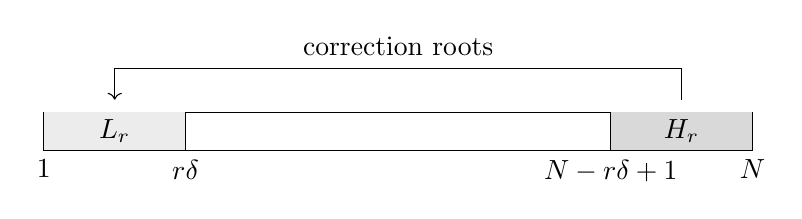
\begin{tikzpicture}[x=0.9cm,y=0.8cm]
 \draw (0,0) rectangle (10,0.6);
 \fill[gray!15] (0,0) rectangle (2,0.6);
 \fill[gray!30] (8,0) rectangle (10,0.6);
 \draw (2,0)--(2,0.6) (8,0)--(8,0.6);
 \node at (1,0.3) {$L_r$};
 \node at (9,0.3) {$H_r$};
 \draw[->] (9,0.8)--(9,1.3)--(1,1.3)--(1,0.8);
 \node at (5,1.65) {correction roots};
 \node[below] at (0,0) {$1$};
 \node[below] at (2,0) {$r\delta$};
 \node[below] at (8,0) {$N-r\delta+1$};
 \node[below] at (10,0) {$N$};
\end{tikzpicture}
\caption{The correction strip goes from the right band
$H_r=\{N-r\delta+1,\ldots,N\}$ to the left band
$L_r=\{1,\ldots,r\delta\}$. Conjugation by one truncated block factor
enlarges each band by at most $\delta$.  Choosing
$N>2(m+1)\delta$ keeps them disjoint throughout the collection.}
\label{kt:strip-figure}
\end{figure}

We claim that conjugating an element of the strip of width
$r\delta$ by one truncated block factor $D_h$, or by its inverse,
keeps it in the strip of width $(r+1)\delta$, whenever $r\leq m$.
It is enough to check a strip root.  Every constituent of $D_h$
goes from an outer index $i$ to a fixed different outer index $j$,
and has inner displacement between $0$ and $d$.  All these
constituents commute.  A constituent initially commuting with the
strip root can therefore be omitted when computing the conjugation:
it also commutes with every conjugate of that root by the other
constituents.

An interacting constituent can change the source endpoint only
when its target is the old source; it then moves that endpoint
left by at most $d$.  It can change the target endpoint only when
its source is the old target; it then moves that endpoint right
by at most $d$.  These assertions, including the coefficients in
their prescribed multiplication order, are precisely the consecutive
Steinberg relations and their reversed versions.  No constituent
can be opposite to a strip root: an edge from its low target to
its high source would have displacement greater than $d$, by the
bound on $N$. This exclusion also holds after one endpoint has moved.
The source inner index minus the target inner index is then greater
than $N-(2r+1)\delta>\delta$, since $r\leq m$ and
$N>2(m+1)\delta$. A constituent of displacement at most $d\leq\delta$
therefore cannot be opposite to an intermediate root.

There is also no accumulation of many shifts at one endpoint during
this single block factor.  After a source change, that source has
outer index $i$, whereas every constituent has target outer index
$j\ne i$, so it cannot change the source again.  After a target
change, that target has outer index $j$, whereas every constituent
has source outer index $i$, so it cannot change the target again.
Both endpoints may change, but each changes at most once.  Every
root produced thus belongs to the strip of width $(r+1)\delta$.
The argument applies to a product of strip roots and to inverse
conjugation as well.  In characteristic two, each block factor is
in fact its own inverse.

Collecting all $D_h$ to the left now gives
\[
 W_v(C_N)=W_v(S_N)\,z,
\]
where $z$ is a product of the wrap factors $F_h$ conjugated by
suffixes of the truncated factors. More explicitly, set
$D_{>h}=D_{h+1}\cdots D_m$ and $D_{>m}=1$. The group identity
\[
 \prod_{h=1}^m(D_hF_h)
 =(D_1\cdots D_m)
   \prod_{h=1}^m(D_{>h}^{-1}F_hD_{>h})
\]
keeps the last product in increasing order of $h$. Thus no correction
factor is used to conjugate another correction. Each suffix has at
most $m$ factors.  The claim puts every resulting correction in the single
strip
\[
 \text{source inner index}>N-(m+1)\delta,
 \qquad
 \text{target inner index}\leq(m+1)\delta.
\]
Its endpoint sets are disjoint by our choice of $N$.  Both evaluated
words have identity matrix image, so $z$ also has identity matrix
image.  Faithfulness of this strip gives $z=1$, as required.
\end{proof}

\subsection{Stable torsion and its descent}

Torsion of nil $K$-groups in positive characteristic is part of the
stable theory
\cite[Corollary~3.3(d)]{Weibel1981}. We make the needed comparison
directly in Steinberg groups and use the rational stability already
proved to descend to the fixed rank.

\begin{proposition}\label{kt:stable-torsion}
Let $n\geq 6$ and $u\in J_n(R)$.  The image of $u$ in
$\St_q(R)$ is torsion for some $q\geq n$ under the standard coordinate
homomorphism.
\end{proposition}

\begin{proof}
Choose a finite root word representing $u$ and apply the grading
homomorphism $\gamma$ to its entries, obtaining the word $u(t)$
from the opening of this section. Its matrix image is the identity,
$u(1)$ represents $u$, and $u(0)$ represents an element of
$J_n(\F_2)$ before the field is included into $R$.

If the word is empty there is nothing to prove.  Otherwise let $m$
be its number of root factors and $d$ the maximum degree of their
entries.  Choose a power of two $N$ with
\[
 N>2(m+1)\max\{1,d\},
\]
and set $W=W_u(C_N)\in\St_{nN}(R)$.

Since $C_N^N=\Id$ and $N$ is a power of two, the binomial identity
in characteristic two gives $(C_N-\Id)^N=0$.  A nilpotent linear
map has an upper triangular matrix with zero diagonal in a basis
adapted to its successive kernels.  Thus some
$P\in\GL_N(\F_2)$ makes $P^{-1}C_NP$ upper triangular with all
diagonal entries equal to $1$.  Lemma~\ref{kt:block-laws} gives
an exact conjugation between the two evaluated root words.  Both
belong to $J_{nN}(R)$, which is central by
Proposition~\ref{prop:centrality}; that conjugation consequently
fixes $W$.  Lemma~\ref{kt:triangular-evaluation} now yields
\[
 W=\prod_{s=1}^{N}\iota_s(u).
\]
Each $\iota_s(u)$ belongs to the central kernel at rank $nN$.
By Lemma~\ref{kt:permutations}, a permutation of coordinates
conjugates any one of these coordinate images to any other.
Centrality therefore makes them equal, and
\begin{equation}\label{kt:cyclic-power}
 W=\iota_1(u)^N.
\end{equation}

On the other hand, Lemma~\ref{kt:wrap-removal} and then
Lemma~\ref{kt:triangular-evaluation}, now with diagonal value $0$,
give
\begin{equation}\label{kt:truncated-power}
 W=W_u(S_N)=\prod_{s=1}^{N}\iota_s(u(0)).
\end{equation}
By Lemma~\ref{kt:field-kernel}, $u(0)$ has finite order.  Its
coordinate images commute, so their product in
\eqref{kt:truncated-power} has finite order as well.  It follows
from \eqref{kt:cyclic-power} that $\iota_1(u)$ has finite order:
if $W^a=1$, then $\iota_1(u)^{Na}=1$.

Finally, a permutation of the $nN$ coordinates carries the ordered
coordinates $(1,1),\ldots,(n,1)$ to the first $n$ usual coordinates.
Lemma~\ref{kt:permutations} identifies $\iota_1(u)$ with a conjugate
of the usual stabilized image of $u$.  Hence that stabilized image
is torsion.  This argument used only coordinate homomorphisms and
never their injectivity.
\end{proof}

\begin{theorem}\label{kt:kernel-torsion}
For every $n\geq 12$, the group $J_n(R)$ is torsion.
\end{theorem}

\begin{proof}
Fix $u\in J_n(R)$ and a homomorphism
$\varphi:J_n(R)\longrightarrow\Q$.  Proposition~\ref{kt:stable-torsion}
provides a rank $q\geq n$ at which the image of $u$ has finite order.
Successively applying Proposition~\ref{prop:rational-stability}
extends $\varphi$ to a homomorphism $J_q(R)\longrightarrow\Q$.
This extension kills the torsion image of $u$, so $\varphi(u)=0$.
The group $J_n(R)$ is abelian by Proposition~\ref{prop:centrality}.
Lemma~\ref{kt:rational-detection} therefore makes $u$ torsion.
Again, no stabilization map was required to be injective.
\end{proof}

\begin{proof}[Proof of Theorem~\ref{thm:main}]
Take the algebra $R$ from Theorem~\ref{thm:algebra} and put
$G=\St_{12}(R)$.  Theorem~\ref{thm:finite-presentation} gives an
ordinary finite presentation of $G$.  Its image $\E_{12}(R)$ is
infinite, because distinct entries in any one elementary matrix
position give distinct matrices and $R$ is infinite.  Thus $G$
is infinite.

By Lemma~\ref{fp:matrix-periodicity}, the elementary matrix group
$\E_{12}(R)$ is periodic.  For $g\in G$, choose a positive integer
$a$ killing its elementary matrix image.  Then $g^a\in J_{12}(R)$,
and Theorem~\ref{kt:kernel-torsion} gives a positive integer $b$
with $(g^a)^b=1$.  Consequently every element of $G$ has finite
order.  The group $G$ is the required infinite, finitely presented
periodic group.
\end{proof}

\subsection{The Kazhdan consequence}\label{sec:kazhdan}

\begin{proof}[Proof of Corollary~\ref{cor:kazhdan}]
Theorem~\ref{thm:algebra} presents \(R\) as a unital associative
\(\F_2\)-algebra on finitely many generators. Since \(\F_2\) is the
prime field, those generators together with \(1\) generate \(R\) as a
ring. Ershov and Jaikin-Zapirain prove that \(\St_n(S)\) has
property~\((T)\) for every finitely generated associative ring \(S\)
with \(1\) and every \(n\geq3\)
\cite[Theorem~6.2]{ErshovJaikinZapirain2010}. This applies directly to
\(S=R\) and \(n=12\). Infinitude, finite presentation, and periodicity
are those of Theorem~\ref{thm:main}.

Write \(G=\St_{12}(R)\). If \(G\) were amenable, normalized
characteristic functions of F\o lner sets would give almost invariant
unit vectors in the left regular representation on \(\ell^2(G)\).
Property~\((T)\) would then give a nonzero invariant vector. Such a
vector is constant on \(G\), and a nonzero constant function on the
infinite group \(G\) is not square-summable. Hence \(G\) is nonamenable.
\end{proof}

\Needspace{20\baselineskip}
\begingroup
\raggedright
\begin{thebibliography}{99}

\bibitem{Burnside1902}
W.~Burnside,
On an unsettled question in the theory of discontinuous groups,
\emph{Quart. J. Pure Appl. Math.} \textbf{33} (1902), 230--238.

\bibitem{Cook1971}
S.~A.~Cook,
The complexity of theorem-proving procedures,
in \emph{Proceedings of the Third Annual ACM Symposium on Theory of
Computing}, ACM, 1971, pp.~151--158.
\url{https://doi.org/10.1145/800157.805047}.

\bibitem{DurandRomashchenkoShen2012}
B.~Durand, A.~Romashchenko, and A.~Shen,
Fixed-point tile sets and their applications,
\emph{J. Comput. Syst. Sci.} \textbf{78} (2012), no.~3, 731--764.
\url{https://doi.org/10.1016/j.jcss.2011.11.001}.

\bibitem{Ershov2008}
M.~Ershov,
Golod--Shafarevich groups with property~$(T)$ and Kac--Moody groups,
\emph{Duke Math. J.} \textbf{145} (2008), no.~2, 309--339.
\url{https://doi.org/10.1215/00127094-2008-053}.
Proposition locator refers to the author version.
\url{https://uva.theopenscholar.com/files/mikhail-ershov/files/gosha_revised4.pdf}.

\bibitem{ErshovJaikinZapirain2010}
M.~Ershov and A.~Jaikin-Zapirain,
Property $(T)$ for noncommutative universal lattices,
\emph{Invent. Math.} \textbf{179} (2010), no.~2, 303--347.
\url{https://doi.org/10.1007/s00222-009-0218-2}.
Theorem locator refers to the author version arXiv:0809.4095v2.
\url{https://arxiv.org/abs/0809.4095v2}.

\bibitem{Golod1964}
E.~S.~Golod,
On nil-algebras and finitely approximable $p$-groups,
\emph{Izv. Akad. Nauk SSSR Ser. Mat.} \textbf{28} (1964), no.~2,
273--276 (Russian).
\url{https://www.mathnet.ru/eng/im2956}.

\bibitem{GolodShafarevich1964}
E.~S.~Golod and I.~R.~Shafarevich,
On the class field tower,
\emph{Izv. Akad. Nauk SSSR Ser. Mat.} \textbf{28} (1964), no.~2,
261--272 (Russian).
\url{https://www.mathnet.ru/eng/im2955}.

\bibitem{IvanovPogodaevKanelBelov2025}
I.~A.~Ivanov-Pogodaev and A.~Ya.~Kanel-Belov,
Construction of a nilsemigroup of paths in a countable family of
uniformly elliptic complexes,
\emph{Algebra and Logic} \textbf{63} (2025), no.~6, 410--438.
\url{https://doi.org/10.1007/s10469-025-09803-3}.

\bibitem{KrsticMcCool}
S.~Krsti\'c and J.~McCool,
\emph{Presenting $\mathrm{GL}_n(k\langle T\rangle)$},
J. Pure Appl. Algebra \textbf{141} (1999), no.~2, 175--183.
\href{https://doi.org/10.1016/S0022-4049(98)00022-X}{doi:10.1016/S0022-4049(98)00022-X}.

\bibitem{Kurosh1941}
A.~G.~Kurosh,
Ringtheoretische Probleme, die mit dem Burnsideschen Problem
\"uber periodische Gruppen in Zusammenhang stehen,
\emph{Izv. Akad. Nauk SSSR Ser. Mat.} \textbf{5} (1941), no.~3,
233--240 (Russian, with German summary).
\url{https://www.mathnet.ru/rus/im3832}.

\bibitem{LenaganSmoktunowiczYoung2012}
T.~H.~Lenagan, A.~Smoktunowicz, and A.~A.~Young,
Nil algebras with restricted growth,
\emph{Proc. Edinb. Math. Soc.} \textbf{55} (2012), no.~2, 461--475.
\url{https://doi.org/10.1017/S0013091510001100}.

\bibitem{NovikovAdian1968}
P.~S.~Novikov and S.~I.~Adian,
Infinite periodic groups. I--III,
\emph{Math. USSR-Izv.} \textbf{2} (1968),
209--236, 241--479, 665--685.
\url{https://doi.org/10.1070/IM1968v002n01ABEH000637}.

\bibitem{OlshanskiiSapir2003}
A.~Yu.~Ol'shanskii and M.~V.~Sapir,
Non-amenable finitely presented torsion-by-cyclic groups,
\emph{Publ. Math. Inst. Hautes \'{E}tudes Sci.} \textbf{96} (2003),
43--169.
\url{https://doi.org/10.1007/s10240-002-0006-7}.

\bibitem{Schutzenberger1961}
M.~P.~Sch\"utzenberger,
On the definition of a family of automata,
\emph{Information and Control} \textbf{4} (1961), nos.~2--3, 245--270.
\url{https://doi.org/10.1016/S0019-9958(61)80020-X}.

\bibitem{Smoktunowicz2008}
A.~Smoktunowicz,
The Jacobson radical of rings with nilpotent homogeneous elements,
\emph{Bull. Lond. Math. Soc.} \textbf{40} (2008), no.~6, 917--928.
\url{https://doi.org/10.1112/blms/bdn086}.

\bibitem{Steinberg1967}
R.~Steinberg,
\emph{Lectures on Chevalley Groups},
notes prepared by J.~Faulkner and R.~Wilson,
Yale University, New Haven, 1967.

\bibitem{vanderKallen1980Homology}
W.~van der Kallen,
\emph{Homology stability for linear groups},
Invent. Math. \textbf{60} (1980), no.~3, 269--295.
\href{https://doi.org/10.1007/BF01390018}{doi:10.1007/BF01390018}.

\bibitem{VasilevYagunov2025Unordered}
I.~Vasilev and S.~Yagunov,
\emph{Unordered resolutions and homological stability for linear groups},
arXiv:2512.18110, 2025.
\href{https://arxiv.org/abs/2512.18110}{arXiv:2512.18110}.

\bibitem{Voronetsky2021Centrality}
E.~Voronetsky,
\emph{Centrality of $K_2$-functor revisited},
J. Pure Appl. Algebra \textbf{225} (2021), no.~4, 106547.
\href{https://doi.org/10.1016/j.jpaa.2020.106547}{doi:10.1016/j.jpaa.2020.106547}.

\bibitem{WeibelKbook}
C.~A.~Weibel,
\emph{The $K$-Book: An Introduction to Algebraic $K$-Theory},
Graduate Studies in Mathematics \textbf{145},
American Mathematical Society, Providence, RI, 2013.

\bibitem{Weibel1981}
C.~A.~Weibel,
\emph{Mayer--Vietoris sequences and module structures on $NK_*$},
in \emph{Algebraic $K$-Theory, Evanston 1980},
Lecture Notes in Mathematics \textbf{854}, Springer, 1981, 466--493.
\url{https://doi.org/10.1007/BFb0089534}.

\bibitem{Weibel1987}
C.~A.~Weibel,
\emph{Module structures on the $K$-theory of graded rings},
J. Algebra \textbf{105} (1987), no.~2, 465--483.
\href{https://doi.org/10.1016/0021-8693(87)90210-9}{doi:10.1016/0021-8693(87)90210-9}.

\bibitem{ZelmanovOdd}
E.~I.~Zel'manov,
Solution of the restricted Burnside problem for groups of odd exponent,
\emph{Math. USSR-Izv.} \textbf{36} (1991), no.~1, 41--60.
\url{https://doi.org/10.1070/IM1991v036n01ABEH001946}.

\bibitem{ZelmanovTwo}
E.~I.~Zel'manov,
A solution of the restricted Burnside problem for $2$-groups,
\emph{Math. USSR-Sb.} \textbf{72} (1992), no.~2, 543--565.
\url{https://doi.org/10.1070/SM1992v072n02ABEH001272}.

\end{thebibliography}

\endgroup
\end{document}
